\documentclass[a4paper,11pt]{report}
\usepackage[T1]{fontenc}
\usepackage[utf8]{inputenc}
\usepackage{lmodern}
\usepackage[english]{babel}
\usepackage[top=3cm,bottom=3cm,left=3.5cm,right=3.5cm]{geometry}
\usepackage{amsmath}
\usepackage{amssymb}
\usepackage{graphicx}
\usepackage{textcomp}
\usepackage{pgf}
\usepackage[siunitx,european]{circuitikz}
\usepackage{etoolbox}
\usepackage{chemfig}
\usepackage{textcomp}
\usepackage{float}
\usepackage{threeparttable}
\usepackage{newfloat}
\usepackage{caption}
\usepackage{hyperref}
%\usepackage[framed,autolinebreaks,numbered]{mcode}
\usepackage{caption}
\usepackage{subcaption}
\usepackage{syntonly}

\usetikzlibrary{patterns}
\usetikzlibrary{fadings}

\DeclareFloatingEnvironment[fileext=frm,placement={!ht},name=Graphe]{graphe}
\captionsetup[graphe]{labelfont=bf}

%\syntaxonly

% \includeonly{
%     Intro_en,
%     Chapitre1_en,
%     Chapitre2_en,
%     Chapitre3_en,
%     Chapitre4_en,
%     Conclu_en,
%     Annexe_en,
%     }
\begin{document}
\begin{titlepage}
\vspace*{\stretch{2}}

    \begin{center}
    
    \hspace*{\stretch{0.2}}
        
\includegraphics[width=45mm]{logo_phelma.png}
        \hfill
        
\includegraphics[width=35mm]{logo_aalto.png}
    \hspace*{\stretch{0.2}}
        \vspace{2cm}
        
        {\LARGE Nicolas \textsc{Paillet}}\\
        \vspace{0.5cm}
        
        \textsc{Course} Physics \& NanoScience (PNS)\\
        Academic year 2014-2015\\
        \vspace{1.5cm}
        
        {\LARGE \textsc{Internship Report}}
        \vspace{0.4cm}
        
        {\Huge \textsc{Fabrication and Measurements}\\        
        \textsc{of NIS junctions to}
        \vspace{0.3cm}
        
        \textsc{characterize Plasma Etching}}     
        
        \vspace{2cm}
        
        Internship realized from the 18$^{th}$ of May 2015 until the 18$^{th}$ of August 2015\\
        
    \vspace{0.3cm}
    
    Within the PICO \textsc{Group}
    \vspace{0.5cm}
    
    
\includegraphics[width=25mm]{logopico.png}
    \vspace{1cm}
    
    \flushleft{
    \textbf{Under the supervision of}\\
    \vspace{0.3cm}
    
    Professor Jukka \textsc{Pekola}, as internship tutor\\
    \textit{jukka.pekola@aalto.fi}\\
    \& \\
    Quentin \textsc{Rafhay}, as school tutor\\
    \textit{quentin.rafhay@phelma.grenoble-inp.fr}\\
    }
    \vspace{0.4cm}
    
    \flushright{Confidentiality : No}
       \end{center} 
    \vspace*{\stretch{3}}
\end{titlepage}
\setcounter{tocdepth}{1}

\pagestyle{empty}
\begin{center}
\vspace*{\stretch{2}}
{\Large \textsc{Aknowledgments}}
\vspace{0.5cm}

\textit{First of all, I would like to thank Pr. Jukka Pekola for having accepted me within the PICO Group and having given me the possibility to do this internship. Of course this would not have been possible without Dr. Clemens Winckelmann who gave me Pr. Pekola contact details. Then, I will of course thank the whole PICO Group for having integrated me so well and helped me when I needed it, but especially Dr. Mathieu Taupin who I worked with on plasma etching project and who gave me precious advices about clean room processes and laboratory methods, alongside with Dr. Matthias Meschke on that last point. Finally, I would like to thank both \textsc{Grenoble INP Phelma} for having given me the opportunity to do such an internship and Aalto University which made it possible afterall.}
\vspace*{\stretch{9}}
\end{center}


\tableofcontents
\thispagestyle{empty}
\setcounter{page}{0}
\pagestyle{fancy}
\chapter*{Glossary}
\addcontentsline{toc}{section}{Glossary}
\textbf{BCS theory : }Theory of superconductivity as explained by Bardeen, Cooper and Schrieffer\\
\textbf{DOS :} Density of electronic states\\
\textbf{EBL :} Electron Beam Lithography\\
\textbf{IVC :} Isolated Vacuum Chamber\\
\textbf{LISA :} Nickname of one of the evaporator in Aalto Nanofab\\
\textbf{MIBK :} Methyl IsoButyl Ketone, a developper\\
\textbf{MMA : } Methyl Methacrilate, a resist\\
\textbf{NIS junction :} Normal metal $-$ Insulator $-$ Superconductor junction\\
\textbf{PMMA :} PolyMethyl Methacrilate, a resist\\


\listoffigures
\addcontentsline{toc}{section}{List Of Figures}

\begin{center}
\vspace*{\stretch{2}}
{\Large \textsc{Aknowledgments}}
\vspace{0.5cm}

\textit{First of all, I would like to thank Pr. Jukka Pekola for having accepted me within the PICO Group and having given me the possibility to do this internship. Of course this would not have been possible without Dr. Clemens Winckelmann who gave me Pr. Pekola contact details. Then, I will of course thank the whole PICO Group for having integrated me so well and helped me when I needed it, but especially Dr. Mathieu Taupin who I worked with on the nanowires project and who gave me precious advices about clean room processes and laboratory methods, alongside with Dr. Matthias Meschke on that last point. Finally, I would like to thank both \textsc{Grenoble INP Phelma} for having given me the opportunity to do such an internship and Aalto University which made it possible afterall.}
\vspace*{\stretch{9}}
\end{center}
\newpage

\section*{The PICO Group}

\indent The PICO Group is a research team which work under the responsibility of the Aalto University School of Science. Its facilities lies in the Micronova building, situated on the Aalto Campus of Otaniemi, in Espoo. Otaniemi is the centre of all scientific activites of the Aalto University and the Micronova building holds the major part of research about nano and microphysics in Finland. The team consists of nineteen members for the moment, including, of course the professor Jukka Pekola, who leads the group and doctor Matthias Meschke who is in charge of the laboratory. Then, the team is divided between five post-doc, seven PhD students and five summer students. 

The Group's researches are varied but especially lies on superconductors properties. The main topics are linked with quantum thermodynamics and single electron transport through nano and microscaled devices. Among the group there are theoretical physicists who focus on the theoretical aspect of research : statistics that rule heat transfert between two nanoscaled resistors\cite{statistics}, for example, whereas some other are focused on practical research : realization of NIS thermometers, electron counting through devices... Moreover, the Group work actively with the Centre for Metrology and Accreditation because one of their main goal is to redefine the ampere, the unit used to measure electrical current\cite{ampere}.

All theses topics of research can be reached thanks to the devices the Group and the building hold. The building owns a clean room, widely used by the members of the Group to make structures. The devices they use are mostly the Electron Beam Lithographier(EBL), evaporators LISA and MASA, and the Scanning Electron Microscope(SEM). The clean room also have devices for making semiconductors-based structures and the Atomic Layer Deposition device was invented here. Then, the Group have a dedicated room in which there are many machines and especially several dilution cryostats. Indeed, since most of the work done within the group has a link with superconductors, they need to reach low temperature to have access to this particular state of matter\cite{NIS_thermo}. There are three regular dilution cryostats that can reach temperature as low as 20mK, and a BlueFors cryostats that works differently but can reach even lower temperatures. In other rooms, there are also devices to characterize and measure : probestation, Atomic Force Microscope (AFM), and SEM, bounders... 

The University and these devices provide the Group the possibility to make research efficiently as we can see the numerous publications published every year in famous journals.


\chapter*{Introduction}
\addcontentsline{toc}{chapter}{Introduction}

Nanostructures are more and more complicated. Researcher in this field always tend to try to make sophisticated devices with many functionalities. This is possible thanks to clean room devices that provide the researchers a way to make more and more different processes. Yet, some of functionnalities in the devices are not well characterized since researchers tend to focus on their actual structures rather than on the characterization of the devices, especially when devices are quite new. However, it is important to have access to all the possibilities that a device offers, this is why it is important to characterize them. 

The evaporator LISA is quite a new device in Micronova's clean room, so that all its functionalities were not characterized, for example it allows plasma etching, which is an \textit{in situ} etching that can be use to get rid of a layer of matter that is not wanted on the structure. But, in order to make this etching reliable, its effect on samples need to be characterized : how does samples react to etching, does etching damage the samples, is the plasma uniform ? All these questions that need answers in order to be able to use the plasma properly.

My role among the group is to make and measure simple structures : Normal Metal-Insulator-Superconductor junction (NIS junction) to determine characterize the plasma etching in an evaporator.

First of all, I will need to understand the theory behind such structures since it is not part of my course, with a literature study (Chapter \ref{Chap1}).

Then, since I will fabricate some structures, I need to know how to do it. I will have trainings to use several devices in the clean room, but I need to understand how they really work, not just knowing on what button to push. Why do we use this device with this particular way to proceed, what are the parameters than have to be taken into account (Chapter \ref{Chap2}). 

Once I know how to the devices work, I need to set some parameters to make consistent measurements and characterize the other parameters with changing only one at a time : I need to build an experimental procedure. I also need to put in place a set up to make measurements : what type of measurements should be done, and how can we measure it (Chapter \ref{Chap3}).

Then, the measurements will give me some datas, which I will need to exploit to turn them into results which I can interpret to understand what happens (Chapter \ref{Chap4}).

\chapter{Theory}
 \label{Chap1}
 
    The first thing to do before starting anything is to understand the goal of the project. For that, it is important to study the behaviour of the structures we want to realize and the physics and quantum phenomemon that can occur. In this chapter we will sum up the litterature study that we have done to understand the theory behind the experiments.
        
        \section{Superconductivity}
            During the research project that Grenoble INP \textsc{Phelma} gave me the opportunity to realize during the first year of my master degree, I have studied superconductors with my group which make this study a bit easier for me since I am familiar with some of the concept mentionned here. Let's start with the basics. 
            Superconductivity is a state of matter which occur mostly at low temperature for several materials. It is a state where the material have an absolute zero resistance, so that current can run without energy losses. It is also a state where the material totally excludes magnetic field and becomes perfectly diamagnetic. These two major properties have a quantum explanation which is the Bardeen-Cooper-Schrieffer(BCS) Theory. Even of this theory does not make unanimity among physicist, since it does not explain everything, it is the most famous at the moment. The qualitative aspect of this theory is quite simple whereas the quantitative involves the second quantization and advanced quantum theories. The eletron within the matter can pair in so-called Cooper pairs which come from an interaction between eletrons an the ion lattice. At low temperature, electron are slow and they tend to attract ions. These ions have a relaxation time to come back to their initial state, but during the time they are in an non-equilibrium state, they create a local positive charge that can attract another electron. This electron is then paired with the previous one. It has the same implusion but an opposite spin according to the BCS Theory. The Cooper pairs, even if formed by two electrons are no longer fermions but bosons so that they follow the Bose-Einstein statistics are form a condensate within the matter. Then, the electrons that are not coupled follow a different density of states where there are two pikes at the distance of $\Delta$, around the energy of the condensate E$_0$ : This is the so-called superconductor gap. Theoretically, the pikes are infinite for a temperature of 0K.
            
        \section{NIS Junctions}
            
        
        \cite{NIS_thermo}
        
        \section{Dilution cryostat}
        
        
        
        %\section{Nanofils semiconducteurs}
        %La physique des nanofils est encore différente de celle des jonctions précédentes. En effet, le projet est basé sur l'utilisation de nanofils d'InAs, qui est semiconducteur. Cependant, celui-ci l'équipe de Copenhague le fait croître epitaxialement à de l'aluminium. Il subit ainsi une supraconductivité de proximité induite par celui-ci. C'est ce phénomène que l'on se propose d'étudier.
        
        %\section{Pompage électronique}
            %A partir des coulomb diamonds, haute fréquence, observation d'un courant d'un seul électron
            \begin{figure}
                \centering
                \begin{tikzpicture}[scale=1.2]
                \draw [->] (0,0)--(10,0);
                \draw (10,0) node[below] {$V_{g}$};
                \draw [->] (0,-3)--(0,3);
                \draw (0,3)node[left]{$V_{bias}$};
                \draw (0,1)--(1,2)--(2,1)--(3,2)--(4,1)--(5,2)--(6,1)--(7,2)--(8,1)--(9,2);
                \draw (0,-1)--(1,-2)--(2,-1)--(3,-2)--(4,-1)--(5,-2)--(6,-1)--(7,-2)--(8,-1)--(9,-2);
                \draw [dashed] (0,-1)--(2,1)--(4,-1)--(6,1)--(8,-1);
                \draw [dashed] (0,1)--(2,-1)--(4,1)--(6,-1)--(8,1);
                
                \draw (3,1)node{$n=0$};
                \draw (5,1)node{$n=1$};
                \draw (7,1)node{$n=2$};
                \draw (1,1)node{$n=-1$};
                \end{tikzpicture}
                
            \caption{Blocage de coulomb dans un supraconducteur et principe du pompage d'électrons}
            \end{figure}
            

\pagestyle{fancy}
\chapter{Experimental methods}
\label{Chap2}
    
    Tools and experimental methods provide the ways to make structures. In this part we will see how the devices and methods used for the process work. In the last part we will talk about the dilution cryostat which was used to cool down samples.

    \section{Resists}
        
        The first part of the process is the deposition of resists on a Silicon wafer with a layer of SiO$_2$.

The resists we use consists of polymer materials : Polymethyl Methacrilate (PMMA) and Methyl Methacrilate (MMA) (See Appendix \ref{appendixresists} Fig. \ref{PMMA}). PMMA is a polymer made out of MMA.
            We depose the resists on the top of the wafer and then a spinner rotates the wafer and makes a thin and uniform layer of resist, with a thickness from 100nm to 500 nm depending on the rotation speed and the type of the resist. In our case, the copolymer thickness is around 400nm.
            
            \begin{figure}
                \centering
                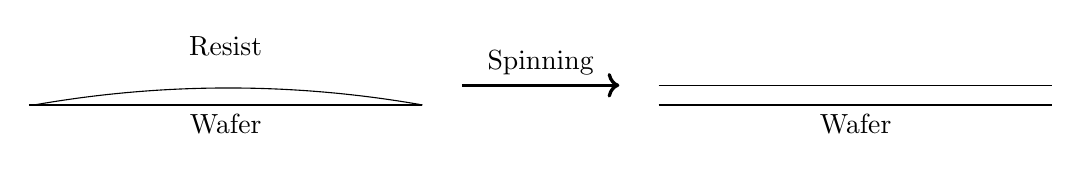
\begin{tikzpicture}
                    \draw [thick] (0,0)--(5,0);
                    \draw (5,0) arc(80:100:14.2);
                    \draw [->, very thick] (5.5,0.25)--(7.5,0.25)node[midway,above]{Spinning};
                    \draw [thick](8,0)--(13,0);
                    \draw (8,0.25)--(13,0.25);
                    \draw (2.5,0)node[below]{Wafer};
                    \draw (10.5,0)node[below]{Wafer};
                    \draw (2.5,0.5)node[above]{Resist};
                \end{tikzpicture}
                \caption{Spinning + Baking}
            \end{figure}
                   
            Practically, we use these two types of resists because they have a different reactivity to the e-beam lithography and to the development process. These two layers have different thicknesses since they do nothave the same role. PMMA acts as a pattern designer, so it cans be thin ($\sim$ 100 - 200nm), whereas we will dig the MMA to create undercuts where the metal will be deposed in the evaporator, this is why the MMA layer needs to be thicker ($\sim$ 1.2$\mu$m), to avoid evaporating on the undercut. 
         Then the resists are baked with a hot plate. The datasheet of the resists can be find in Ref. \cite{Datasheet}. We finally obtain the cross-section shown in Fig. \ref{resine}.
            
            \begin{figure}
                \centering 
                \begin{tikzpicture}
                    \draw (0,0)--(10,0);
                    \draw (5,-0.5) node{Wafer $Si/SiO_2$};
                    \draw (0,2)--(10,2);
                    \draw (5,1)node{MMA};
                    \draw (0,2.5)--(10,2.5);
                    \draw (5,2.25) node{PMMA};
                \end{tikzpicture}
                \caption{Cross-section view after resist deposit, spinning and baking}
                \label{resine}
            \end{figure}
            
                        
            The resists we use are sensitive to electrons with a particular energy, what we will do next is to expose the resist to an electron beam (See \ref{explicationebl}) which will imply structural modifications. The electrons break the polymer into smaller pieces, which make the exposed resist more soluble in Methyl IsoButyl Ketone (MIBK) (See \ref{development}).
            
              Other type of resists exists, especially some resists damaged by light (photoresits), which are mostly used for semiconductors-based structures.
              
    \section{Electron Beam Lithography and development}
        
        Once the wafer have been prepared and is covered by resists, we can draw a pattern in these resists, with the Electron Beam Lithography (EBL).
        
        \subsection{Electron Beam Lithography}
            The EBL is a tool which is used to design the patterns we want to have for our structures\cite{EBL_theory}. It sends an electron beam onto the resist to damage the bonds of the resist, making the exposed area sensitive to the development process. The functionnal diagram can be found in Appendix \ref{appendixEBL} Fig. \ref{EBLschema}.The E-beam lithography gives the opportunity to make very small structures, down to few tens of nanometer in size with a resolution of few nanometers. The drawback of such low resolution is the writing time, a compromise between good accuracy and reasonable writing time has thus to be found.
            
            For example, the only part that requires an good accuracy in our process is the junction, so we have to use a good resolution there, but for the leads, which are much larger when the actual size does not matter, so we can choose to go faster. 
            In addition to the primary electrons from the beam, the resist is also affected by the secondary elestrons, backscattered from the substrate. These electrons will create a wider exposed area below the PMMA and is called "undercut" (See Fig. \ref{waferEBL}). This is this undercut that give the possibility to shadow evaporation (see below).
            
            \label{explicationebl}
                    
            \begin{figure}
                \centering
                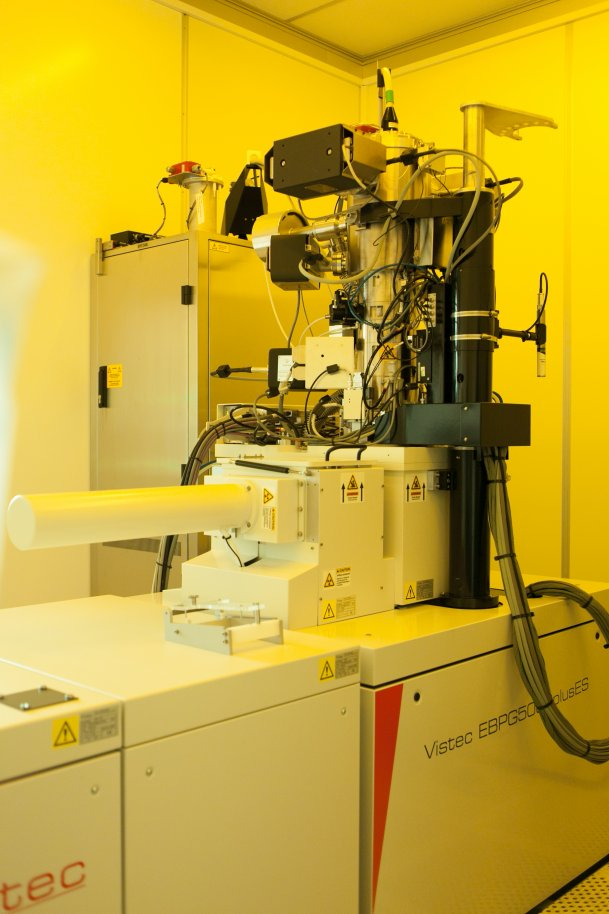
\includegraphics[width=100pt]{EBL.jpg}
                \caption{Electron Beam Lithographier Vistec of Micronova cleanroom}
            \end{figure}
            
            Once the wafer has been exposed, it can be represented by Fig \ref{waferEBL}.
                    
            \begin{figure}
                \centering
                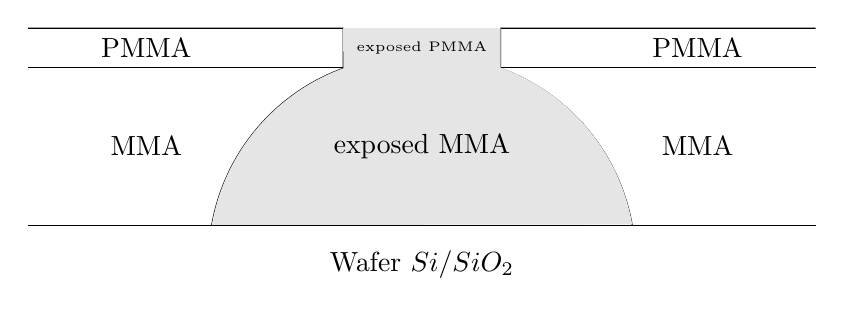
\begin{tikzpicture}
                \draw (0,0)--(10,0);
                \draw (5,-0.5) node{Wafer $Si/SiO_2$};
                \draw (2.33,0) arc(170:110:2.6)--(4,2.5)--(0,2.5);
                \draw (7.67,0) arc(10:70:2.6)--(6,2.5)--(10,2.5);
                \fill [color=gray!20](2.33,0) arc(170:110:2.6)--(4,2.5)--(6,2.5)--(6,2) arc(70:10:2.6);
                \draw (0,2)--(4,2);
                \draw (6,2)--(10,2);
                \draw (1.5,1) node{MMA};
                \draw (8.5,1) node{MMA};
                \draw (1.5,2.25) node{PMMA};
                \draw (8.5,2.25) node{PMMA};
                \draw (5,2.25)node{{\tiny exposed PMMA}};
                 \draw (0,0)--(10,0);
                \draw (5,1)node{exposed MMA};
                \end{tikzpicture}
                \caption{Cross-section view after EBL}
                \label{waferEBL}
            \end{figure}
        
        \subsection{Development}
        
            \label{development}
            The Development consists in the withdrawal of the exposed resit. It is realized by chemical reactions.
            
            
            %Our goal is to make junction between Al and Cu, if we depose Al or Cu on this wafer, they will depose everywhere and we will just have Aluminium covered by Copper. To make a junction, we need a way to not depose metal everywhere. This is the role of the undercuts and evaporation angles (See \ref{evapangles}).
            
            The MIBK(See Appendix \ref{appendixresists} Fig. \ref{MIBK}) will dissolve fastly the exposed PMMA and MMA (Fig. \ref{aprèsMIBK}).If we want to increase the width of the undercut, it is possible to add an extra step and to use MethylGlycol after the development in MIBK. The MethyGlycol can dissolve MMA and thus increase the undercut \cite{methylglycol}. This is particularly useful if we want to work with large angles.
            
            There, we can see that if we depose metal with a certain angle, they will overlap only in the chosen area. Finally, we dive the sample in Isopropanol to stop the reaction.

The dissolution will depend on the time we dive the samples into the chemicals, we need to chose this time considering the width of the undercuts but ensure that PMMA does not collapse.
            
            \begin{figure}
                \centering
                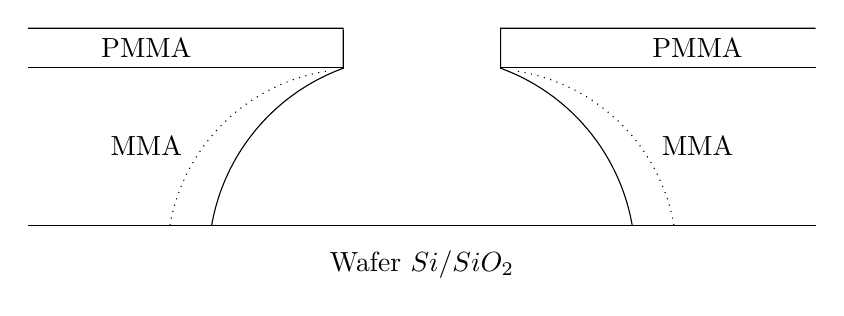
\begin{tikzpicture}
                \draw (0,0)--(10,0);
                \draw (5,-0.5) node{Wafer $Si/SiO_2$};
                \draw (2.33,0) arc(170:110:2.6)--(4,2.5)--(0,2.5);
                \draw (7.67,0) arc(10:70:2.6)--(6,2.5)--(10,2.5);
                \draw [dotted](1.8,0) arc(170:98:2.4);
                \draw [dotted] (8.2,0) arc(10:82:2.4);
                \draw (0,2)--(4,2);
                \draw (6,2)--(10,2);
                \draw (1.5,1) node{MMA};
                \draw (8.5,1) node{MMA};
                \draw (1.5,2.25) node{PMMA};
                \draw (8.5,2.25) node{PMMA};
                \end{tikzpicture}
                \caption{Cross-section view after MIBK (full lines), and after MethyGlycol (dotted lines)}
                \label{aprèsMIBK}
            \end{figure}
            
    \section{Evaporation}
        During the evaporation step, we make the junctions by evaporating metal.
        
        \subsection{Functioning of evaporator}
        
        The evaporator is a tool that allows to deposit a uniform, thin layer of metal. A filament is submitted to a large tension (10kV) and current, it emits electrons that are deflected with a magnetic field to focus on a crucible which contains metal. The metal will melt, or even sublimate, depending on the metal. The atoms can move without collision in the very low pressure chamber ($P\sim10^{-7}mbar$) : the mean free path is longer ($\sim$ 1km) than the distance between the crucible and the sample holder ($\sim$ 50cm). The deposition of the atoms is very uniform and the thickness is measured with capacitive sensors.
        The chamber of the evaporator is connected to a pure Oxygen line, in order to perform oxidation \textit{in situ}. The most common superconductor used is Al, and its oxidation is very rapid (an exposure of 2mbar of O$_2$ during 2 minutes is enough to create a tunnel barrier).
        
        \subsection{The Plasma gun}
        
        The evaporator is also equipped with a Plasma Gun, with Argon valve. The plasma is mostly used at low power to ease the lift-off (See \ref{lift-off}) by weakening the resist and to clean the surface. But with the accurate parameters it can also be used for etching. The idea of plasma etching is to etch native oxide of a material, which has been grown in another process, so exposed to air, and to make contact in a controlled way (clean contact or tunnel barrier).
        
        %One of the goals of this project is to characterize this technique in the evaporator here : characterize the plasma and determine its effect on samples (See \ref{Chap3}). We need to know better about plasma etching because the nanowires will come from Copenhaguen and the Aluminium layer will be strongly oxidized, thing that we do not want. We will need to get rid of it one way or another, this is why we try plasma etching. We will realize different junctions with different plasma parameters to know better how it behaves.         
            
            \begin{figure}
                \centering
                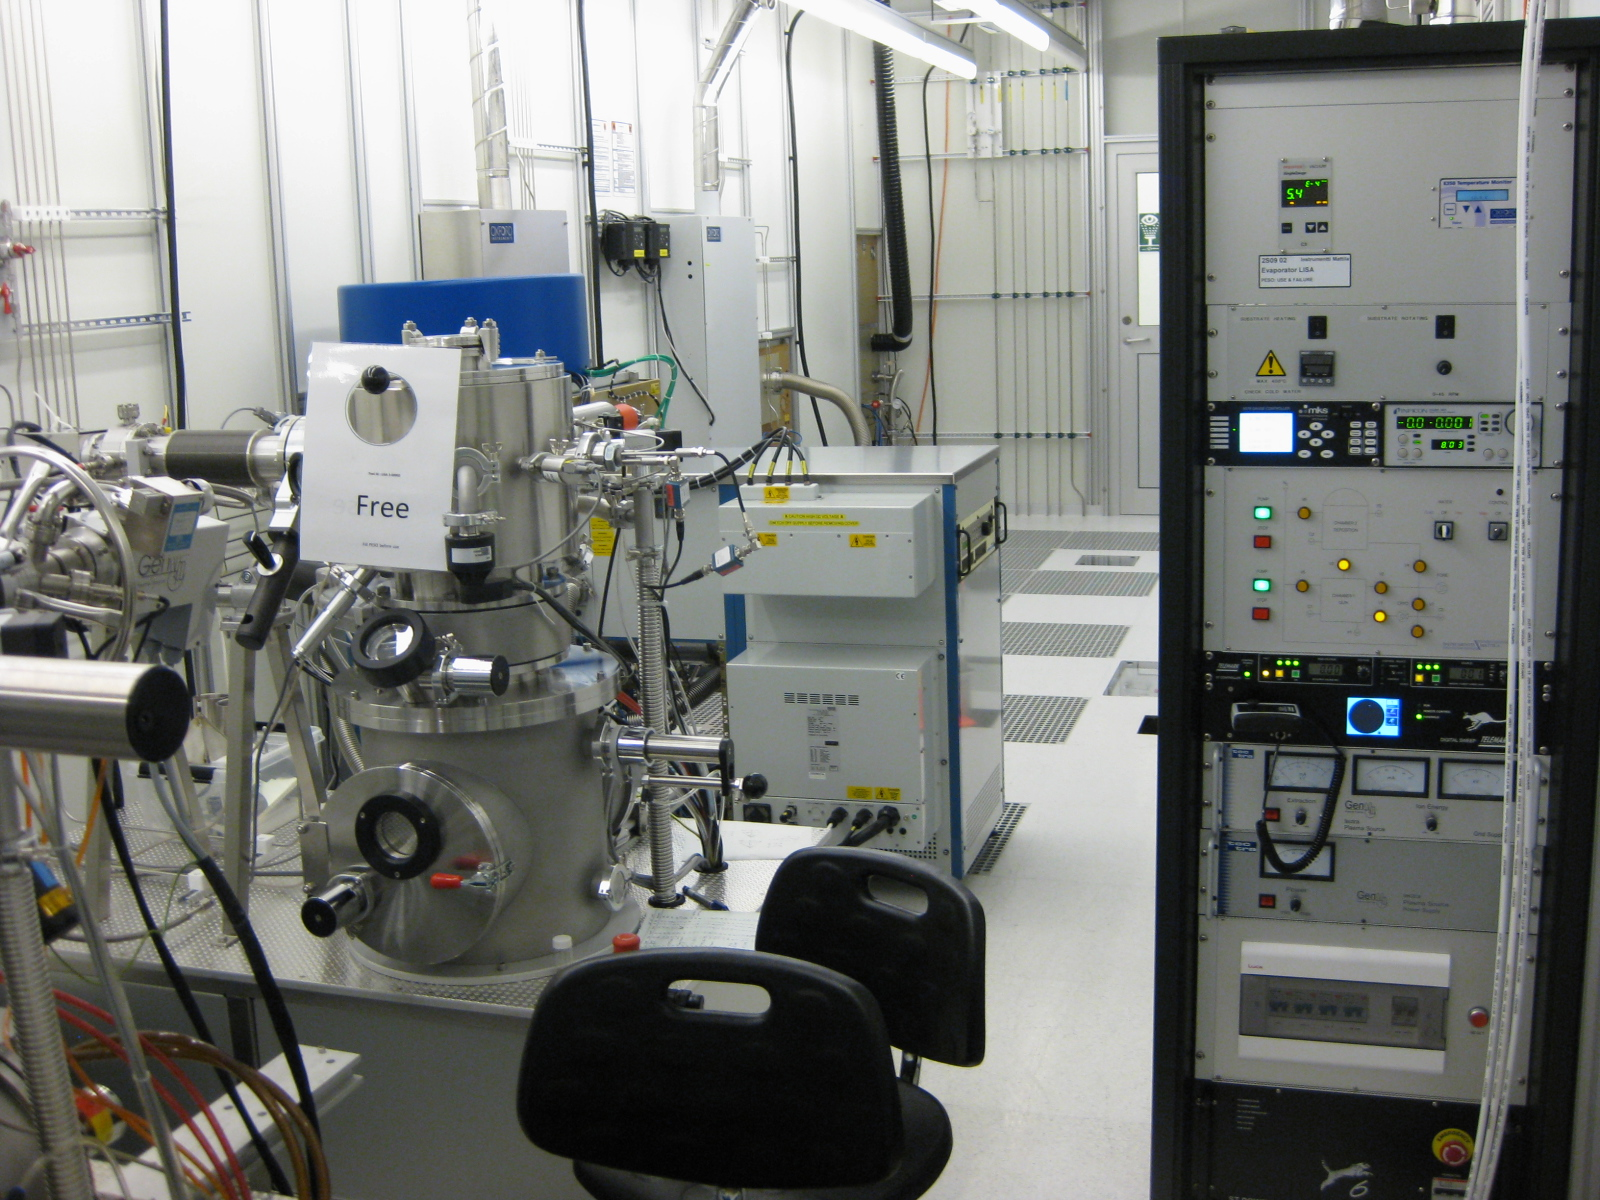
\includegraphics[width=200pt]{LISA.JPG}
                \caption{Picture of the LISA evaporator in Micronova cleanroom}
            \end{figure}
            
            
            \subsection{Evaporator in action}
            
                \label{evapangles}
                The Fig. \ref{evaporation} shows the principle of evaporation. First, we depose the first layer of metal with a previously determined angle. If needed, it is possible to oxidize to obtain a tunnel barrier, then another layer is evaporated, with another angle. The pattern and the angles are such that only the active parts (the junctions) will overlap. Thus, we can see that even it they are in the same undercut, they do not touch each other. To make the junction, we have to have two different undercuts that overlap.
                
            \begin{figure}
            \centering
            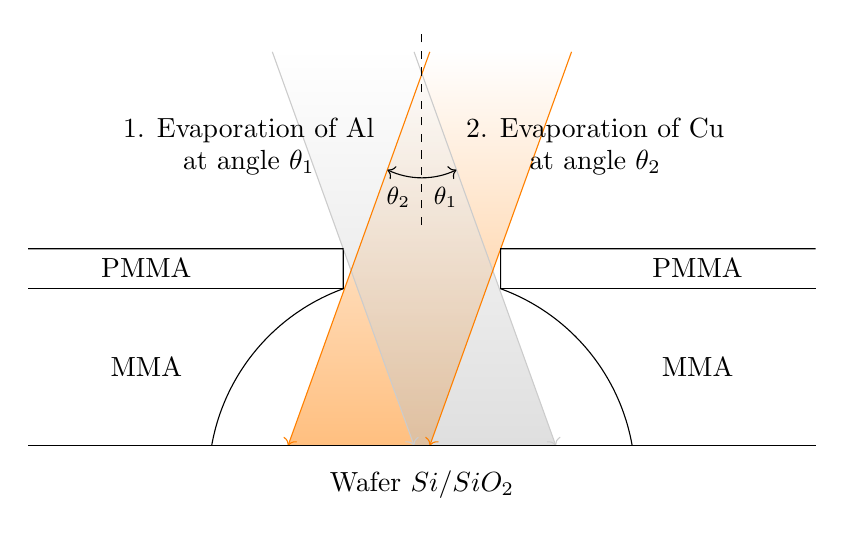
\begin{tikzpicture}
                
                \shadedraw[bottom color=orange,top color=white, draw=orange, fill opacity=0.5,draw opacity=0](5.1,5)--(3.3,0)--(5.1,0)--(6.9,5)-- cycle;
                \shadedraw[bottom color=gray!50,top color=white, draw=gray!40, fill opacity=0.5, draw opacity=0](4.9,5)--(6.7,0)--(4.9,0)--(3.1,5)--cycle;   
                \draw [color=gray!40,->] (4.9,5)--(6.7,0);
                \draw [color=gray!40,->] (3.1,5)--(4.9,0);  
                \draw [color=orange,->] (5.1,5)--(3.3,0);
                \draw [color=orange,<-] (5.1,0)--(6.9,5);
                          
                \draw (0,0)--(10,0);
                \draw (5,-0.5) node{Wafer $Si/SiO_2$};
                \draw (2.33,0) arc(170:110:2.6)--(4,2.5)--(0,2.5);
                \draw (7.67,0) arc(10:70:2.6)--(6,2.5)--(10,2.5);
                \draw (0,2)--(4,2);
                \draw (6,2)--(10,2);
                \draw (1.5,1) node{MMA};
                \draw (8.5,1) node{MMA};
                \draw (1.5,2.25) node{PMMA};
                \draw (8.5,2.25) node{PMMA};
                \draw [dashed](5,2.8)--(5,5.3);
                \draw [->] (5,3.4) arc(-90:-116:1);
                \draw (2.8,4) node{1. Evaporation of Al};
                \draw(2.8,3.6) node{at angle $\theta_1$} ;               
                \draw (4.7,3.4)node[below]{{\small $\theta_2$}};
                \draw [->] (5,3.4) arc(-90:-64:1);
                \draw (7.2,4)node {2. Evaporation of Cu};
                \draw (7.2,3.6)node{at angle $\theta_2$};
                \draw (5.3,3.4)node[below]{{\small $\theta_1$}};
                
            \end{tikzpicture} 
            \caption[Cross-section during evaporation]{Cross-section during evaporation (the two metal are evaporated succesively, not at the same time)}
            \label{evaporation}
            \end{figure}
        
                
                
                
    \section{Lift-off and Scanning Electron Microscope}

        \subsection{Lift-off : resist withdrawal}
        \label{lift-off}
        
            The lift-off is a process where the resist is removed to get our final structures. The chip is dived into an acetone bath, which will dissolve the resist and left on the substrate only the device made.
            
        \subsection{Scanning Electron Microscope}
            The functioning of Scanning Electron Microscope (SEM) is very similar to the EBL one, since actually, SEM and EBL are the same instrument, except that this time we do not want to weaken the matter but to observe the scattering of electrons within it. This allows us to check if the junctions made looks measureable, if metals evaporated overlap in the chosen area, meaning that the angle is correct. It is useful for a process that is not completely established, where the angles, or the EBL electron dose are still to be improved.
            
            \begin{figure}
                \centering
                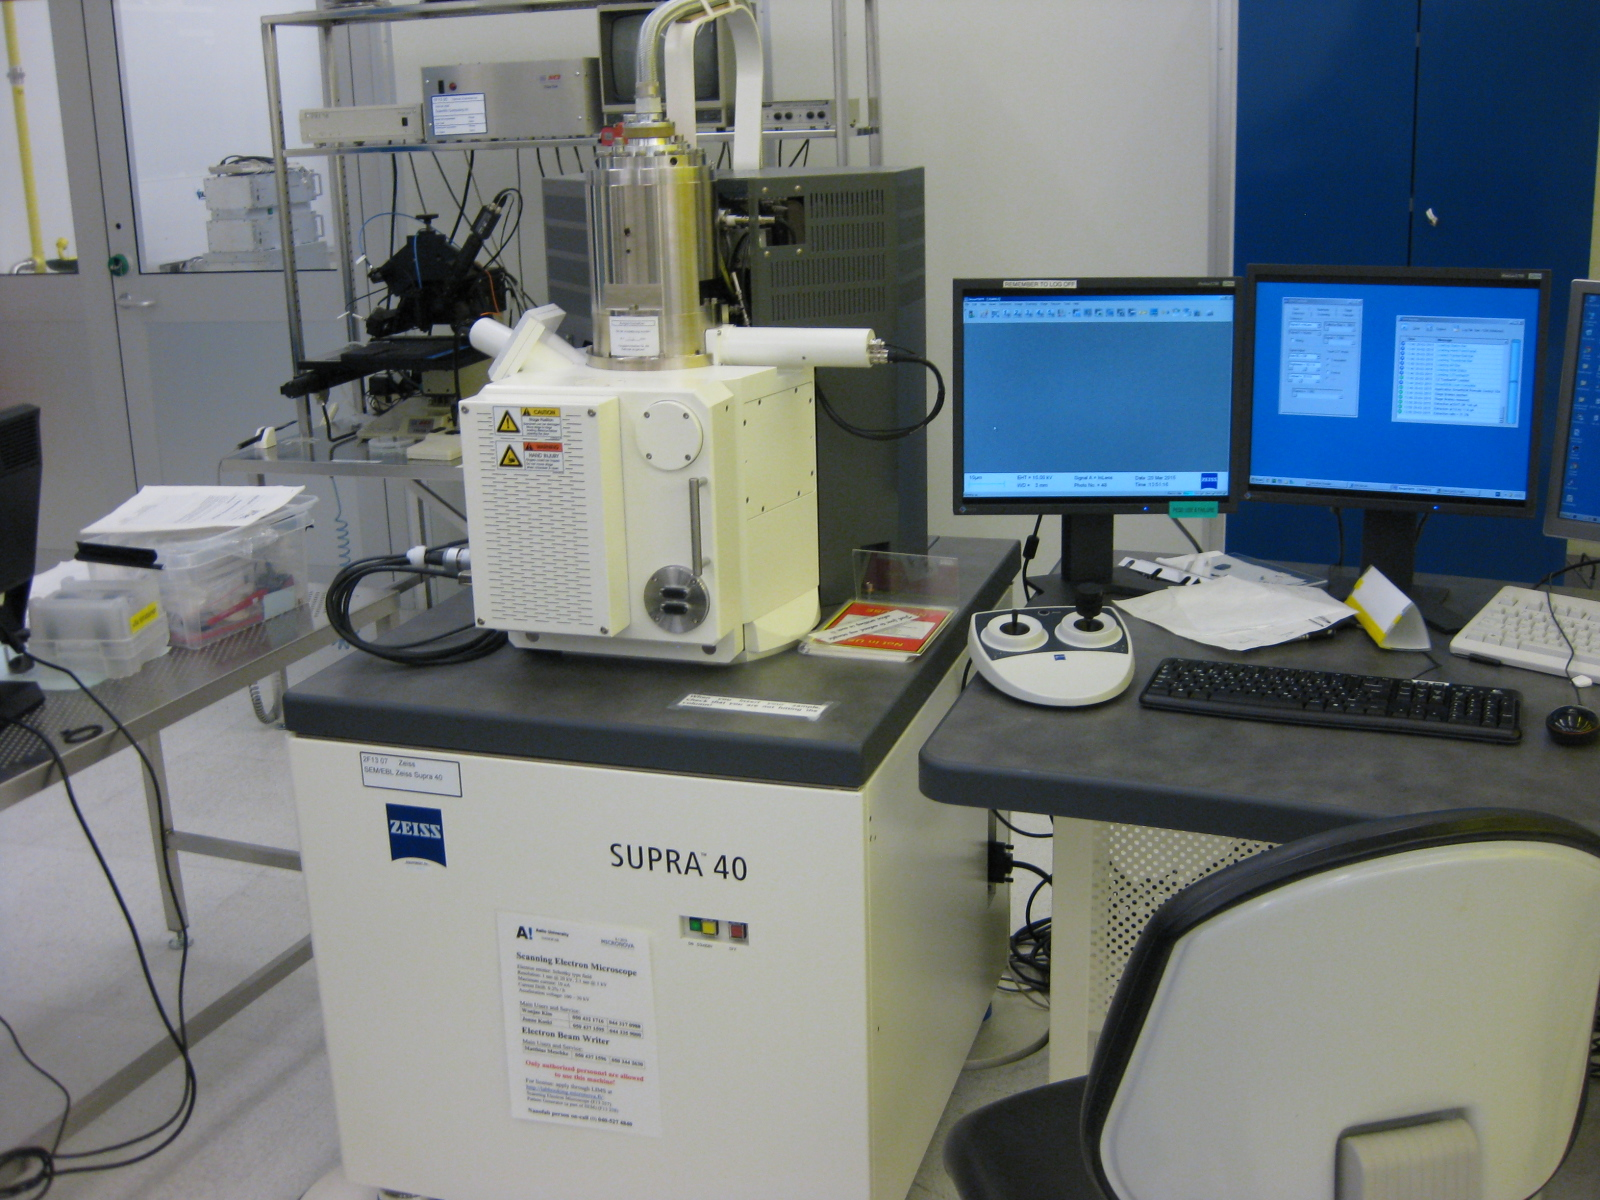
\includegraphics[width=200pt]{SEM.JPG}
                \caption{Scanning Electron Microscope}
            \end{figure}
            
        \subsection{Observation of the samples}
            The SEM is very similar to an optical microscope, in the way that the clarity of the image will depend on the focusing of the beam on the sample, except that it is not light here but electrons. This can be problematic as it can be possible to charge the objects observed if the beam stays too long on the same spot, and this can damage the junctions, especially if they are small.
            
            As in the EBL, the matter scatters the electron, especially metals. These scattered electrons can be detected with the secondary electron mode. Since each metal scatters electrons in a different way, in this mode will only the metals appear and different contrasts allow to distinguish them, despiting the brightness and quality of the signal (few scattered electrons inducing noise).
            
            %requires some adjustments in order to give us good images. The settings look very like optical settings : focus, stigmatism, aperture... To set them, we first choose a place where there is no samples, in order to avoid to charge them since we send electron within the matter. Of course, if there is nothing at all, it will be very difficult to set anything, so we choose a place with metal but which does not belong to a structure. Once the location chosen, we have to set the different parameters to get the best image possible. We align both focus and stigmation together by adjusting, and zooming when we have the optimal settings. The more we zoom in, the more tricky it becomes to get a good image. 
            
            A typical SEM image is shown in Fig. \ref{SEMexemple} and an image with the secondary electron mode of SEM is shown in Fig. \ref{SEMexemplese2}. As said before, the SEM can show some problems with the juntions, like in Fig. \ref{SEMexemplefail}. In our case, a chip contains 20 devices. It is not necessary to image all of them, only a few are sufficient, as the real test to determine the quality of the device is the measurement of the resistance.
            
            
             \begin{figure}
        \centering
            \begin{subfigure}[t]{0.48\textwidth}
                \centering
                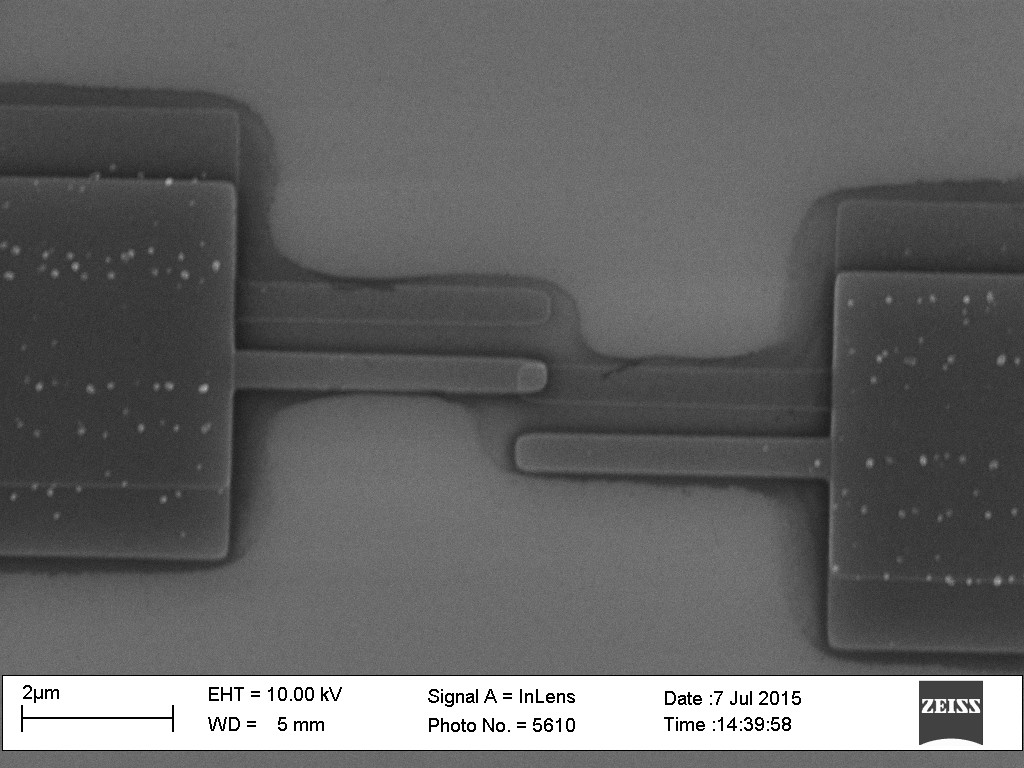
\includegraphics[width=180pt]{SEMexemple.jpg}
                \caption{SEM image of a sample in normal mode}
                \label{SEMexemple}
                \end{subfigure}
                ~
                \begin{subfigure}[t]{0.48\textwidth}
                \centering
                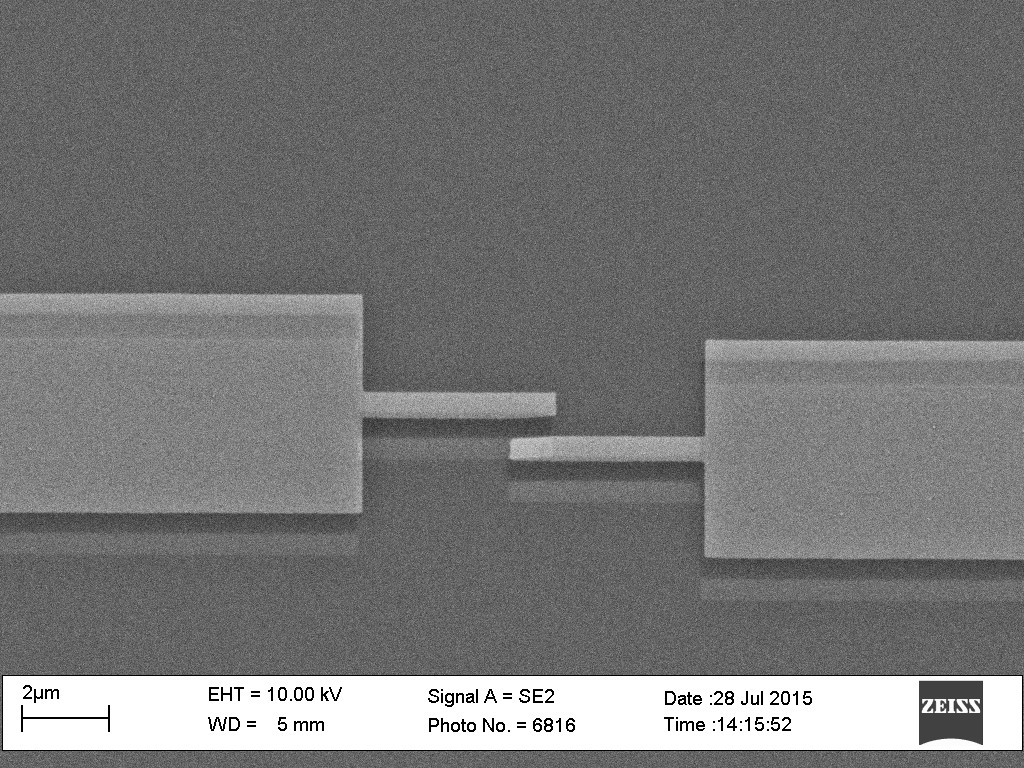
\includegraphics[width=180pt]{SEMexemplese2.jpg}
                \caption{SEM image of a sample in secondary electron mode}
                \label{SEMexemplese2}
                \end{subfigure}
                
                \begin{subfigure}[t]{0.99\textwidth}
                \centering
                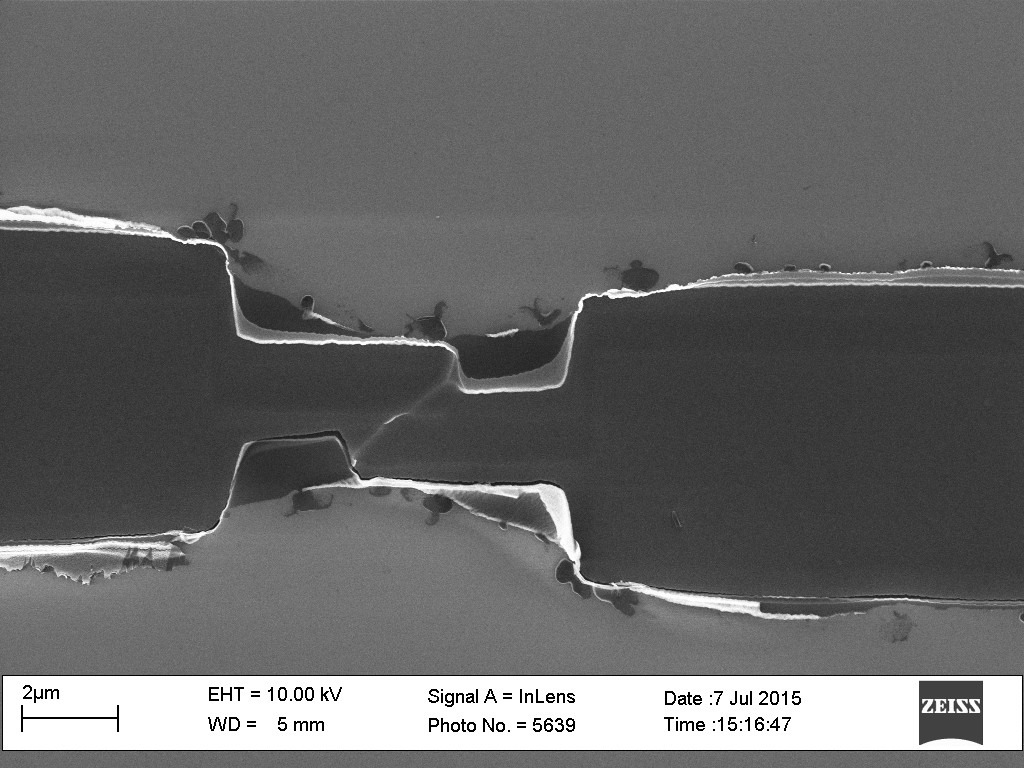
\includegraphics[width=250pt]{SEMexemplefail.jpg}
                \caption{SEM image of a failed sample}
                \label{SEMexemplefail}
                \end{subfigure}
            \end{figure}
            
            
            \section{Dilution cryostat}
            
            \subsection{Cooling theory}    
            The $^4$He is liquid at a temperature of 4.2K. The minimum reachable temperature with $^4$He is 1.2K and 0.3K for the $^3$He by pumping. In order to reach lower temperatures, we use a mixture of $^3$He/$^4$He, where the temperature can be as low as 3mK in the best fridges. The phase diagram of the $^3$He/$^4$He mixture is shown in Fig. \ref{phasediagram} : with 10-15\% of $^3$He, a phase separation will occur below 0.5K due to the existence of a "forbidden zone" in the diagram. We will thus have a rich phase (of $^3$He) and a diluted phase. 
        
        \begin{figure}
            \centering
            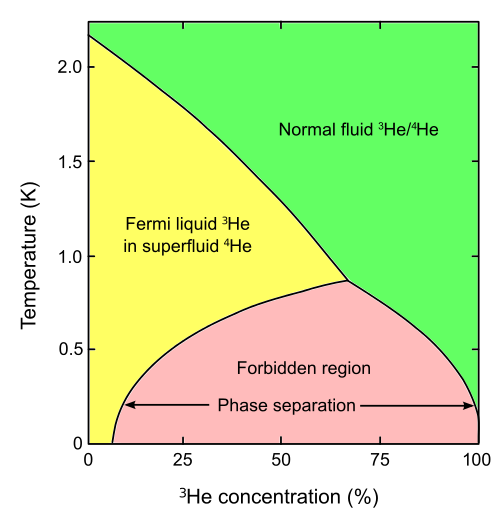
\includegraphics[width=200pt]{phasediagram.png}
            \caption{Phase diagram of $^3$He/$^4$He mixture}
            \label{phasediagram}
        \end{figure}
        
The whole cooling power lies in this phase separation \cite{fridge}. The mixture goes through a 77K nitrogen trap, in order to be cleaned of any impurities, then a line run through the fridge towards the $^4$He bath at 4.2K then to a 1K pot (pumped $^4$He bath). This bath liquefies the mixture which then goes to an exchanger, the still that cools down to 600mK, and ends up in the mixing chamber where the phase separation occurs which has for effect to remove heat from the mixing chamber environment. The mixture is pumped back out of the fridge and injected again through the condensing line, as a close loop.

            \subsection{Preparation of the sample}
            
            The first thing to do with low temperature measurements is to prepare the sample to get in the fridge. Sample holder consists in metallic pads linked to a 12-pins connector. The sample is bounded to the sample holder with thin Al wires with an ultrasound bounder (Fig. \ref{bounding}). The sample holder is screwed to the fridge (Fig. \ref{screwstage}) and sealed in the vacuum chamber (IVC). 
               
               \begin{figure}
                    \centering
                    \begin{subfigure}[t]{0.48\textwidth}
                    \centering
                    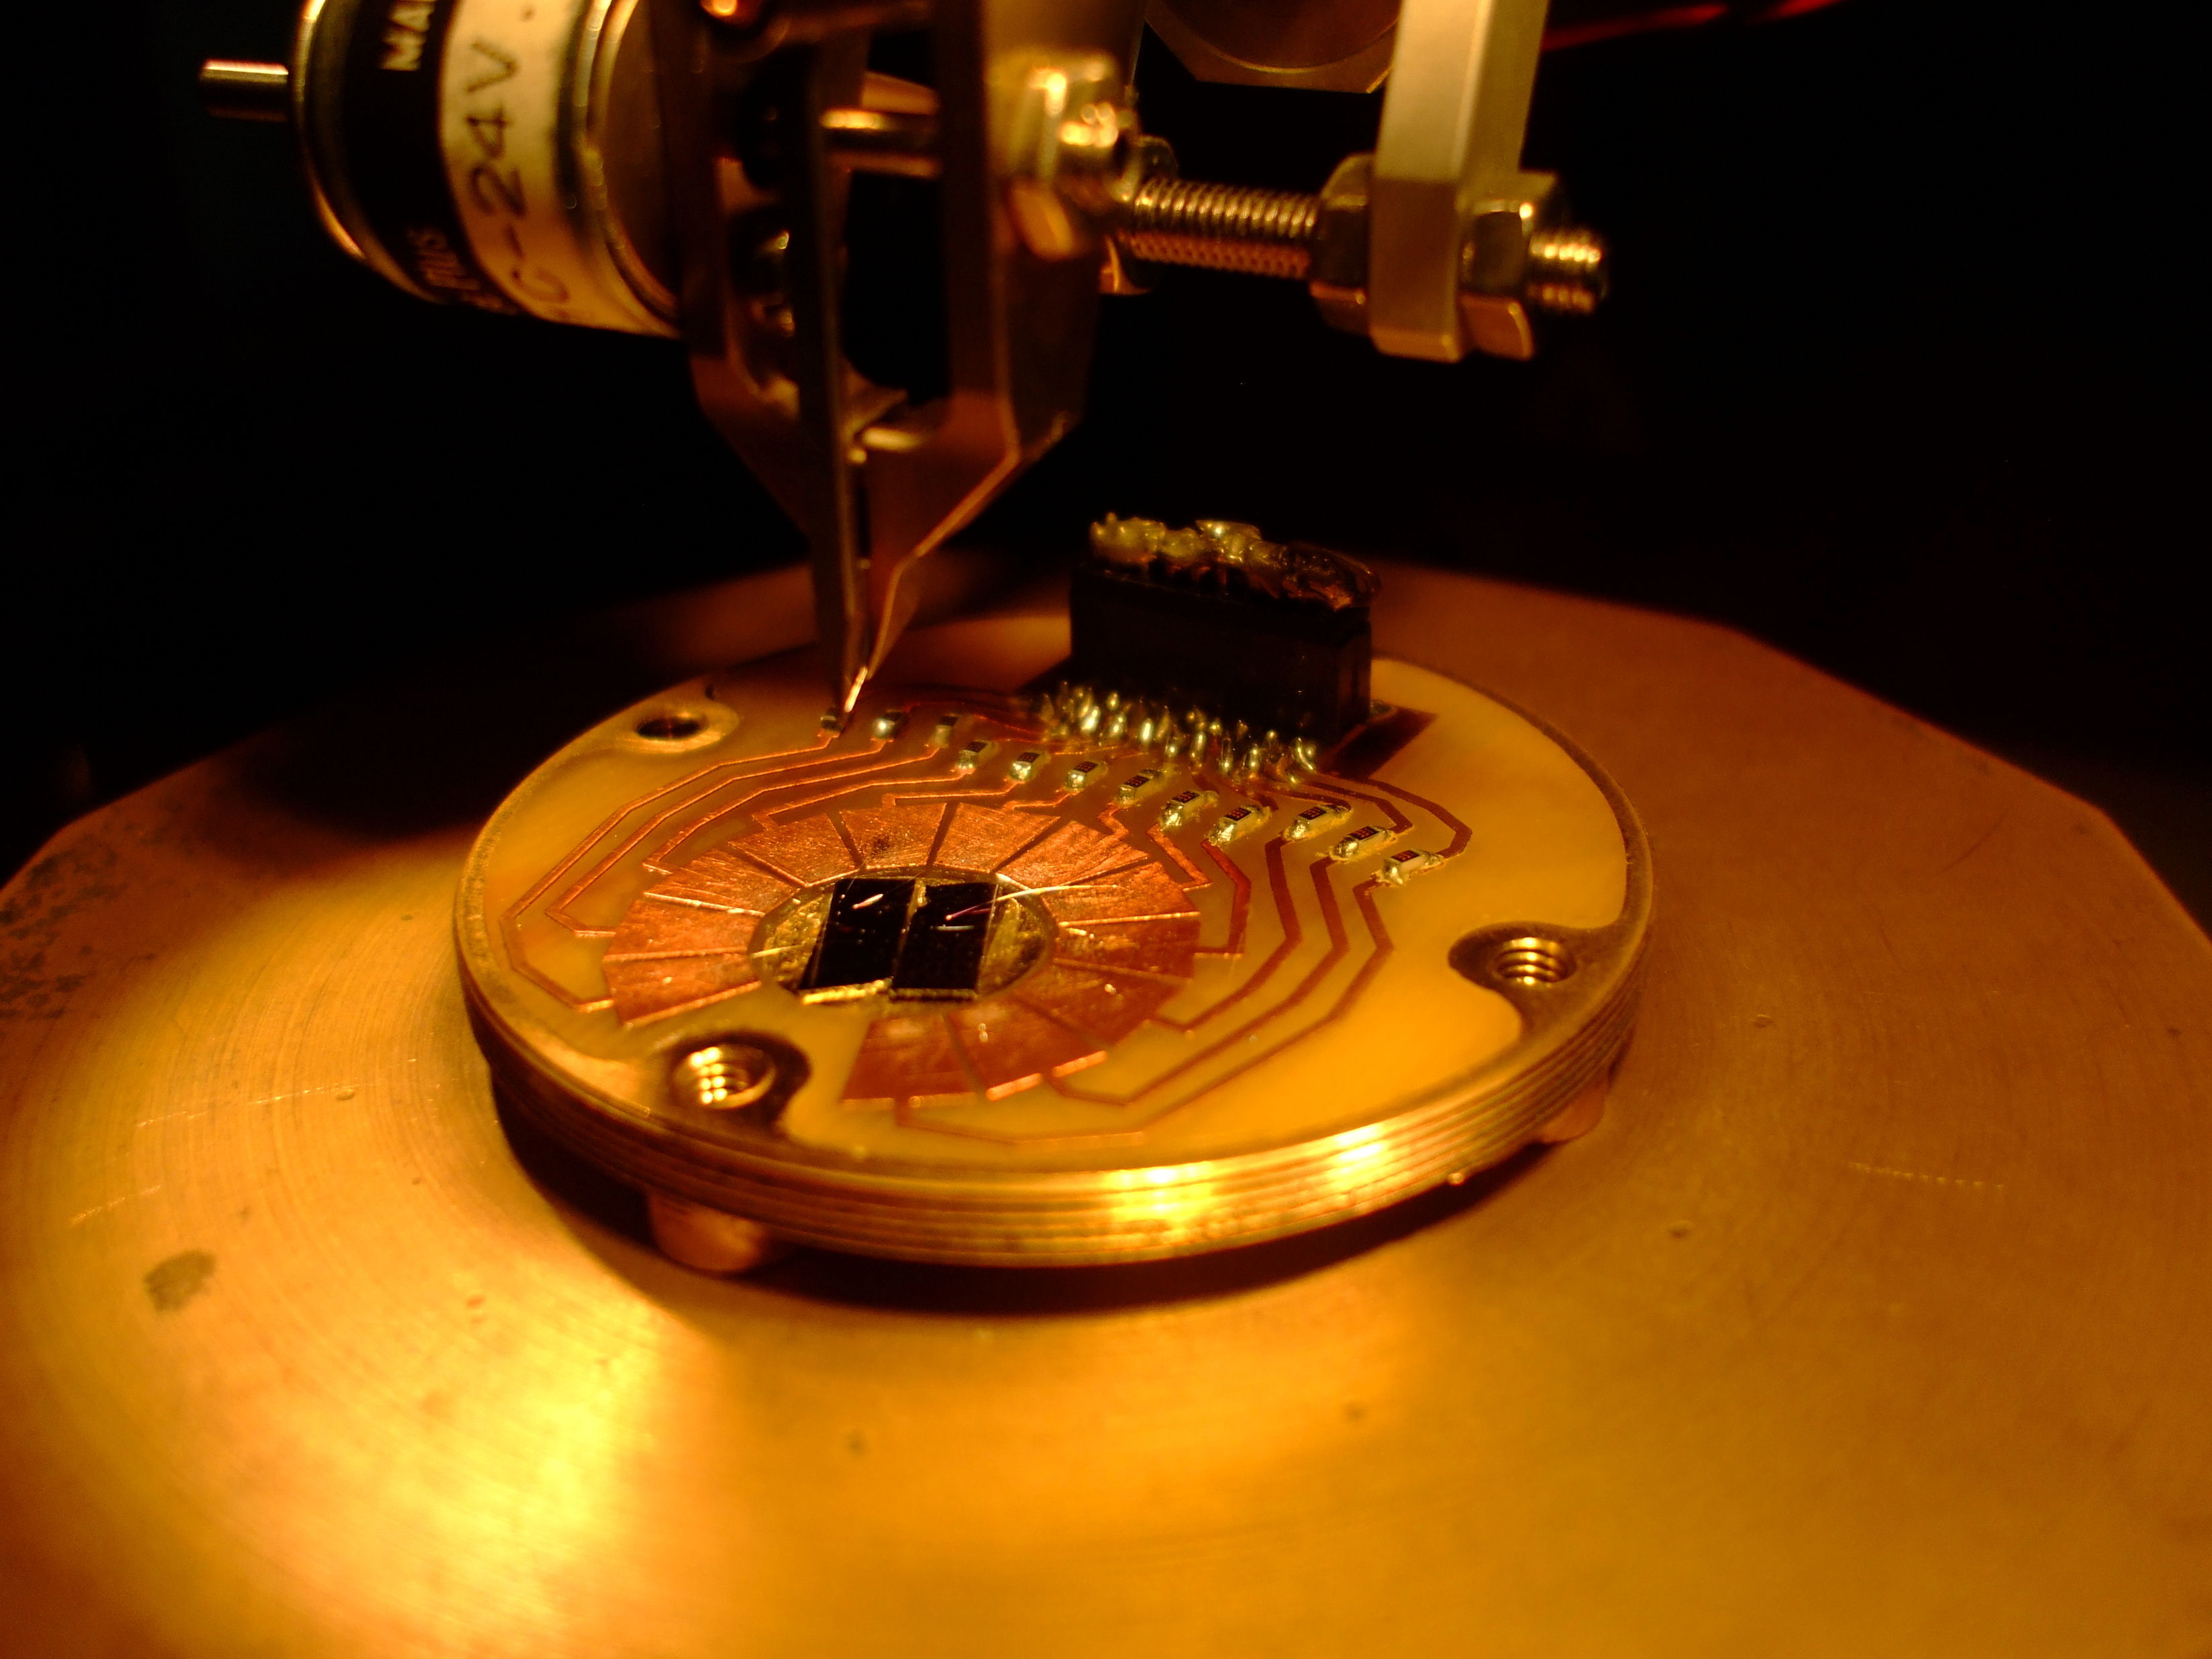
\includegraphics[width=6cm]{bounding.JPG}
                    \caption{Picture of the sample stage}
                    \label{bounding}
                    \end{subfigure}  
                    \begin{subfigure}[t]{0.48\textwidth}
                    \centering
                    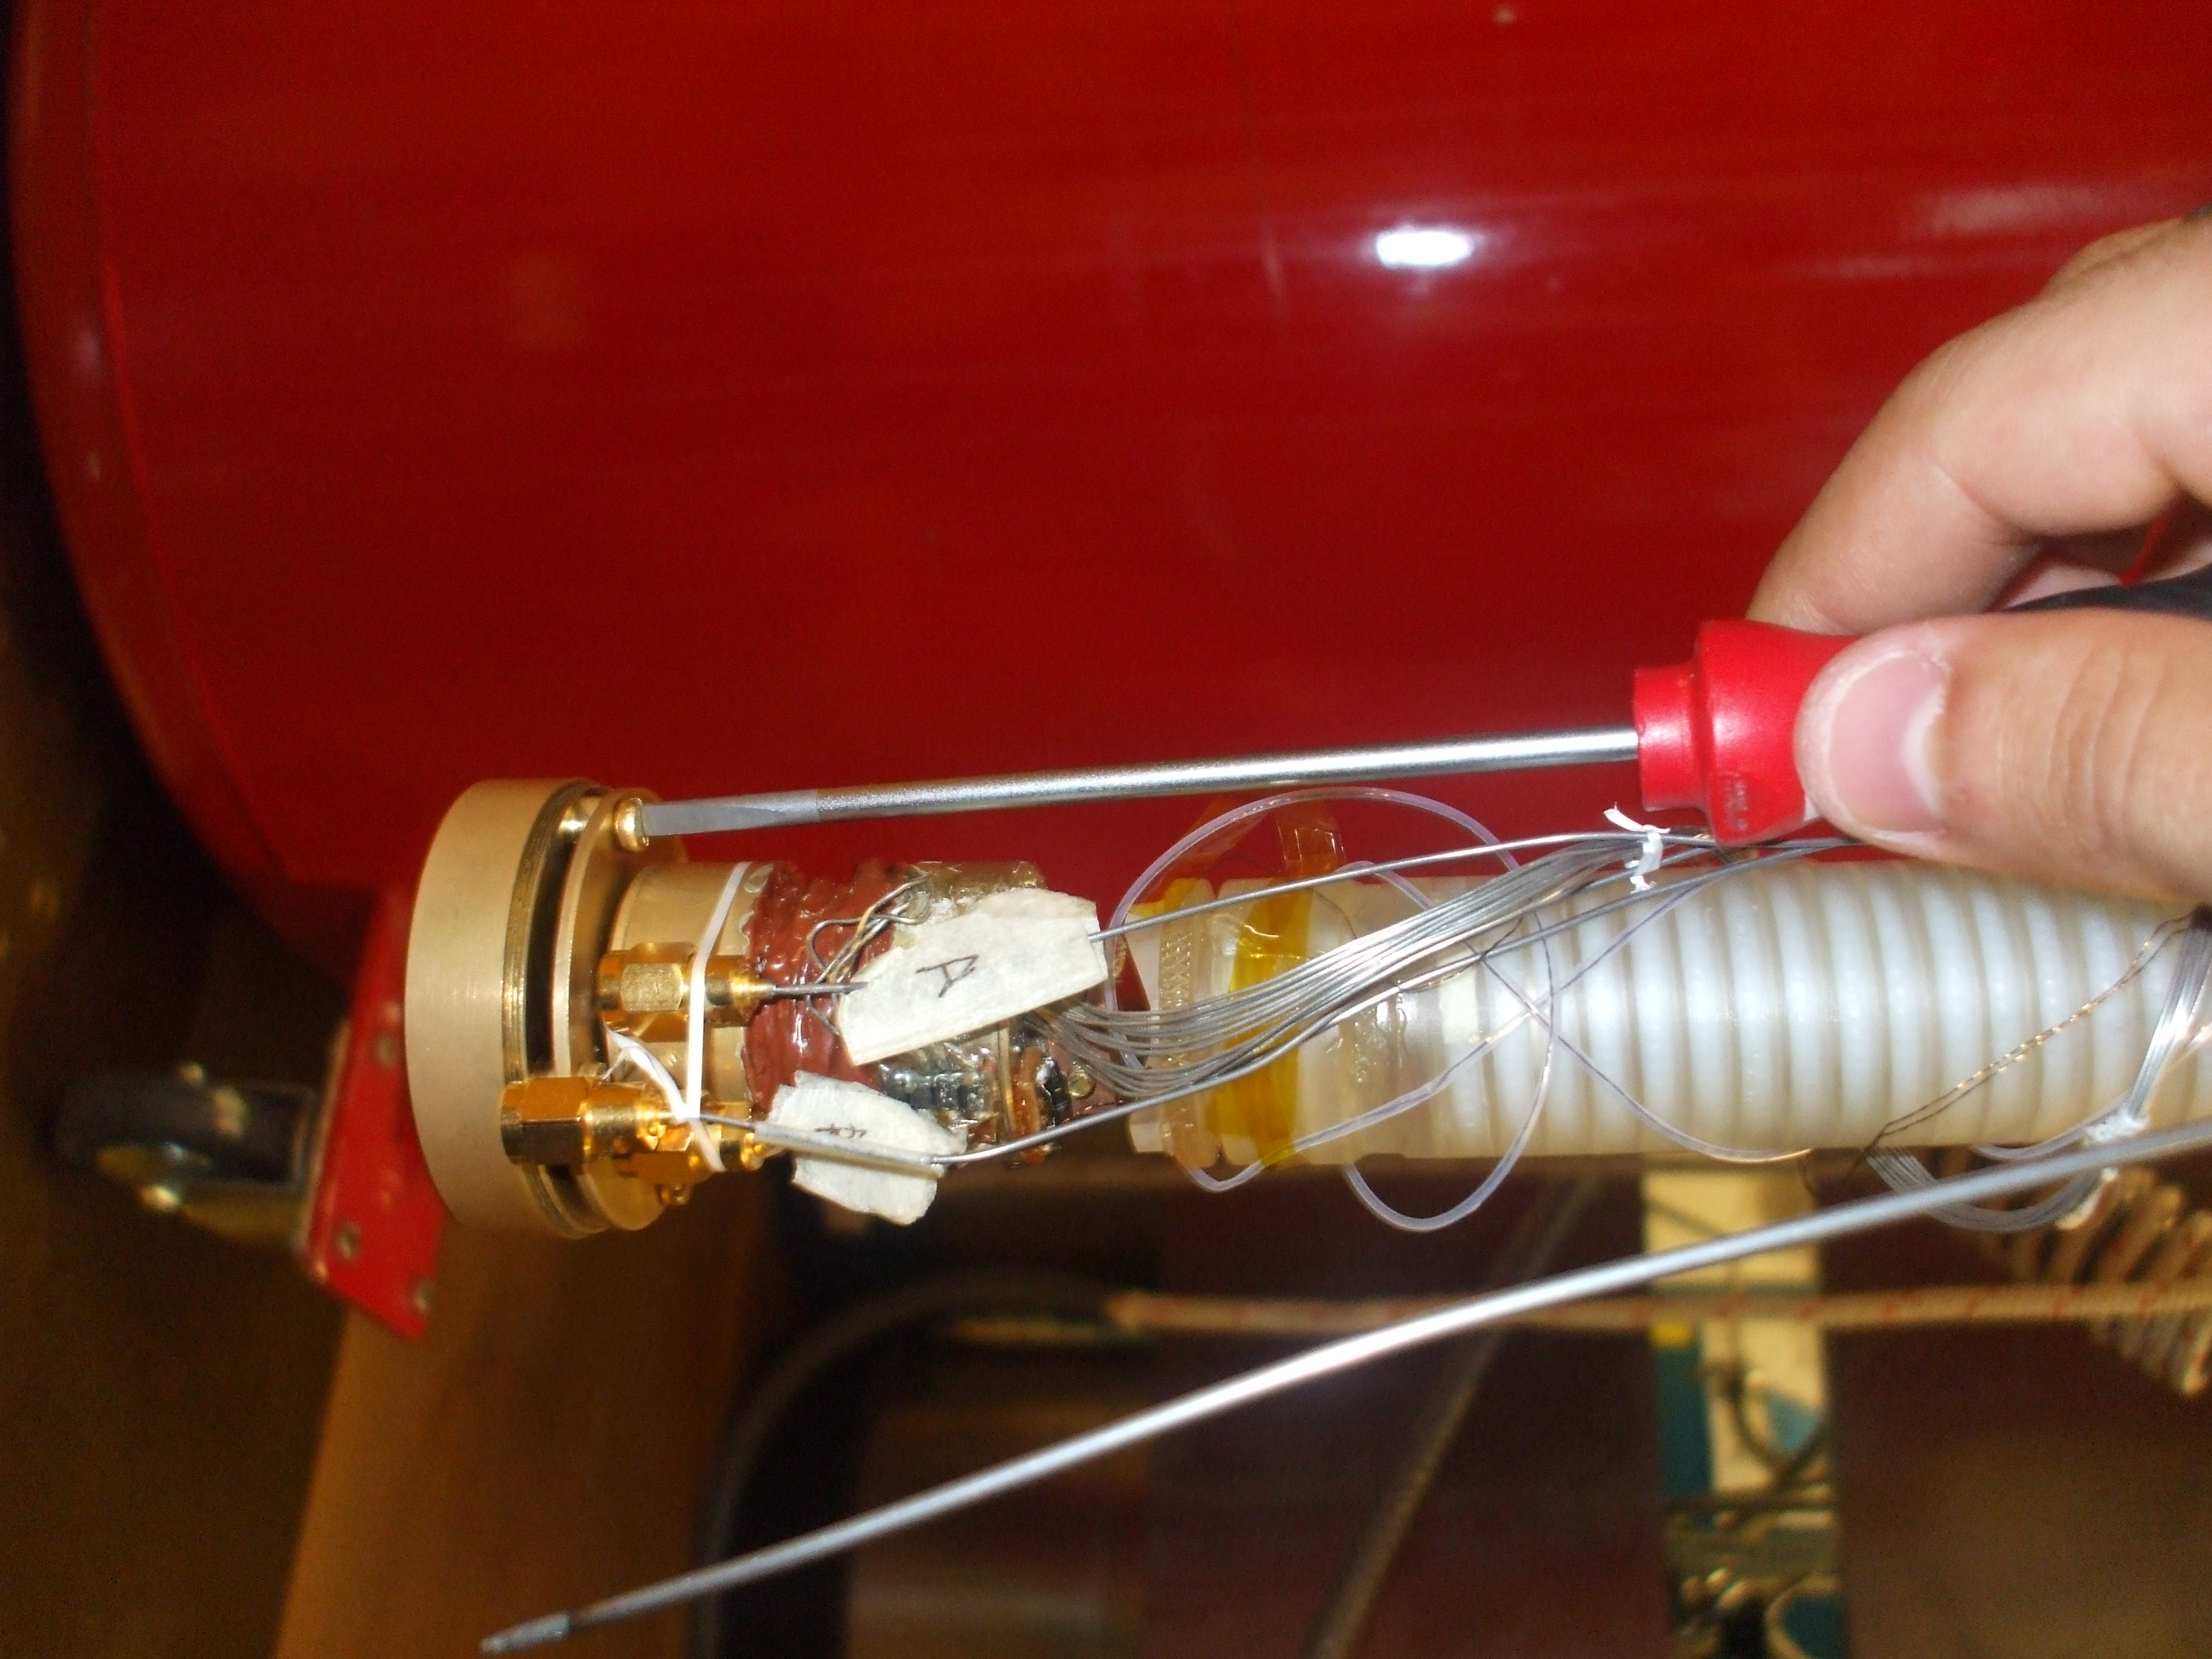
\includegraphics[angle=90,width=5cm]{screwstage.JPG}
                    \caption{Exchanger and mixing chamber with the sample holder}
                    \label{screwstage}
               \end{subfigure}   
               \caption{Pictures of the preparation of the sample stage}         
                \end{figure}
                       
          
            
            \subsection{Cooling down}
            
            The first step of the cooling is to pump the Isolated Vacuum Chamber (IVC) to remove all the air from it and avoid any freezing. Then, some exchange gas (Helium) is inserted into the dilution, in order to reduce the thermal conductivity that exists between the stages of the fridge. The gas will cool down the dilution by convection. The fridge is then placed in a nitrogen bath (Fig. \ref{nitrogen}) during approximatively thirty minutes before diving it in the Helium dewar. The goal is to avoid to evaporate Helium in the dewar (the difference between 77K and 4K is less important and Nitrogen can be cooled more easily). Once the fridge is thermalized at 4K (Fig. \ref{Setup4K}), checked by RuO$_2$ thermoresistor, the exchange gas is pumped back to avoid heat transfert by convection, otherwise the fridge can not be cooled down to 50mK. Finally, the mixture is inserted in the fridge and starts to circulate, like in Fig. \ref{loopmixture}
            
            
            \begin{figure}
            \begin{subfigure}[t]{0.48\textwidth}
            \centering
                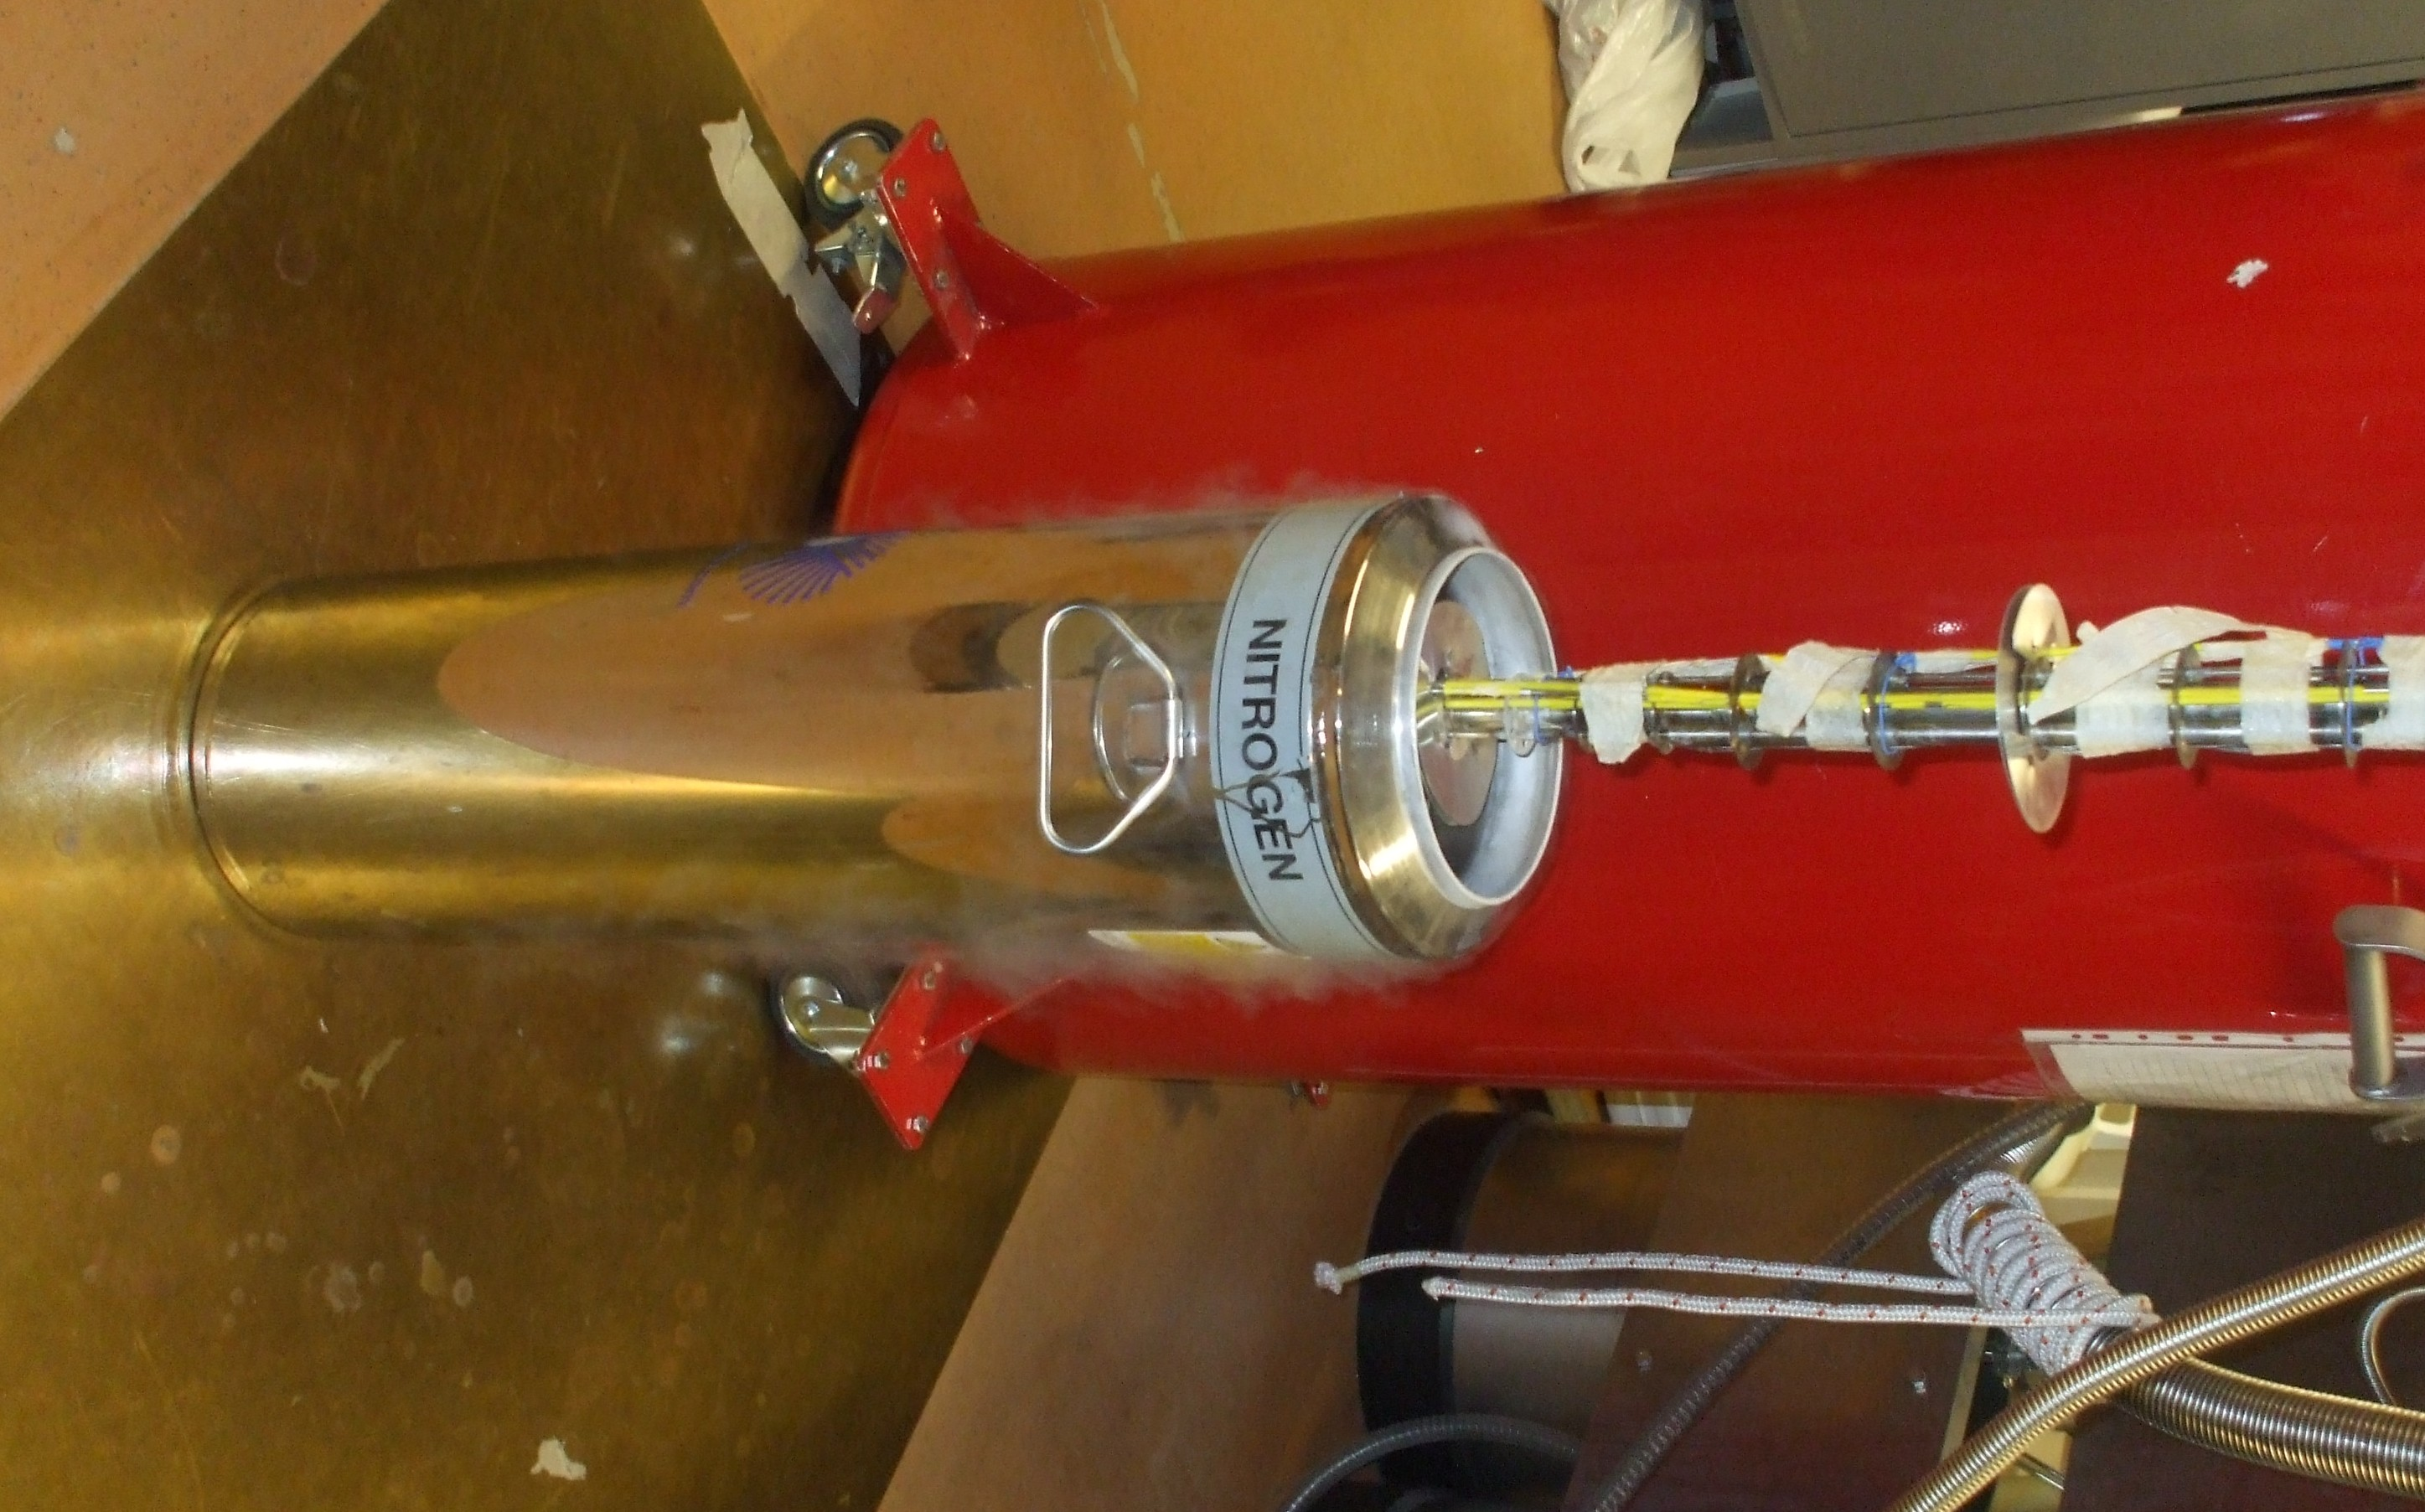
\includegraphics[angle=90,width=4.5cm]{nitrogen.JPG}
                \caption{Picture of the IVC dived into liquid nitrogen}
                \label{nitrogen}
            \end{subfigure}
             \begin{subfigure}[t]{0.48\textwidth}
             \centering
                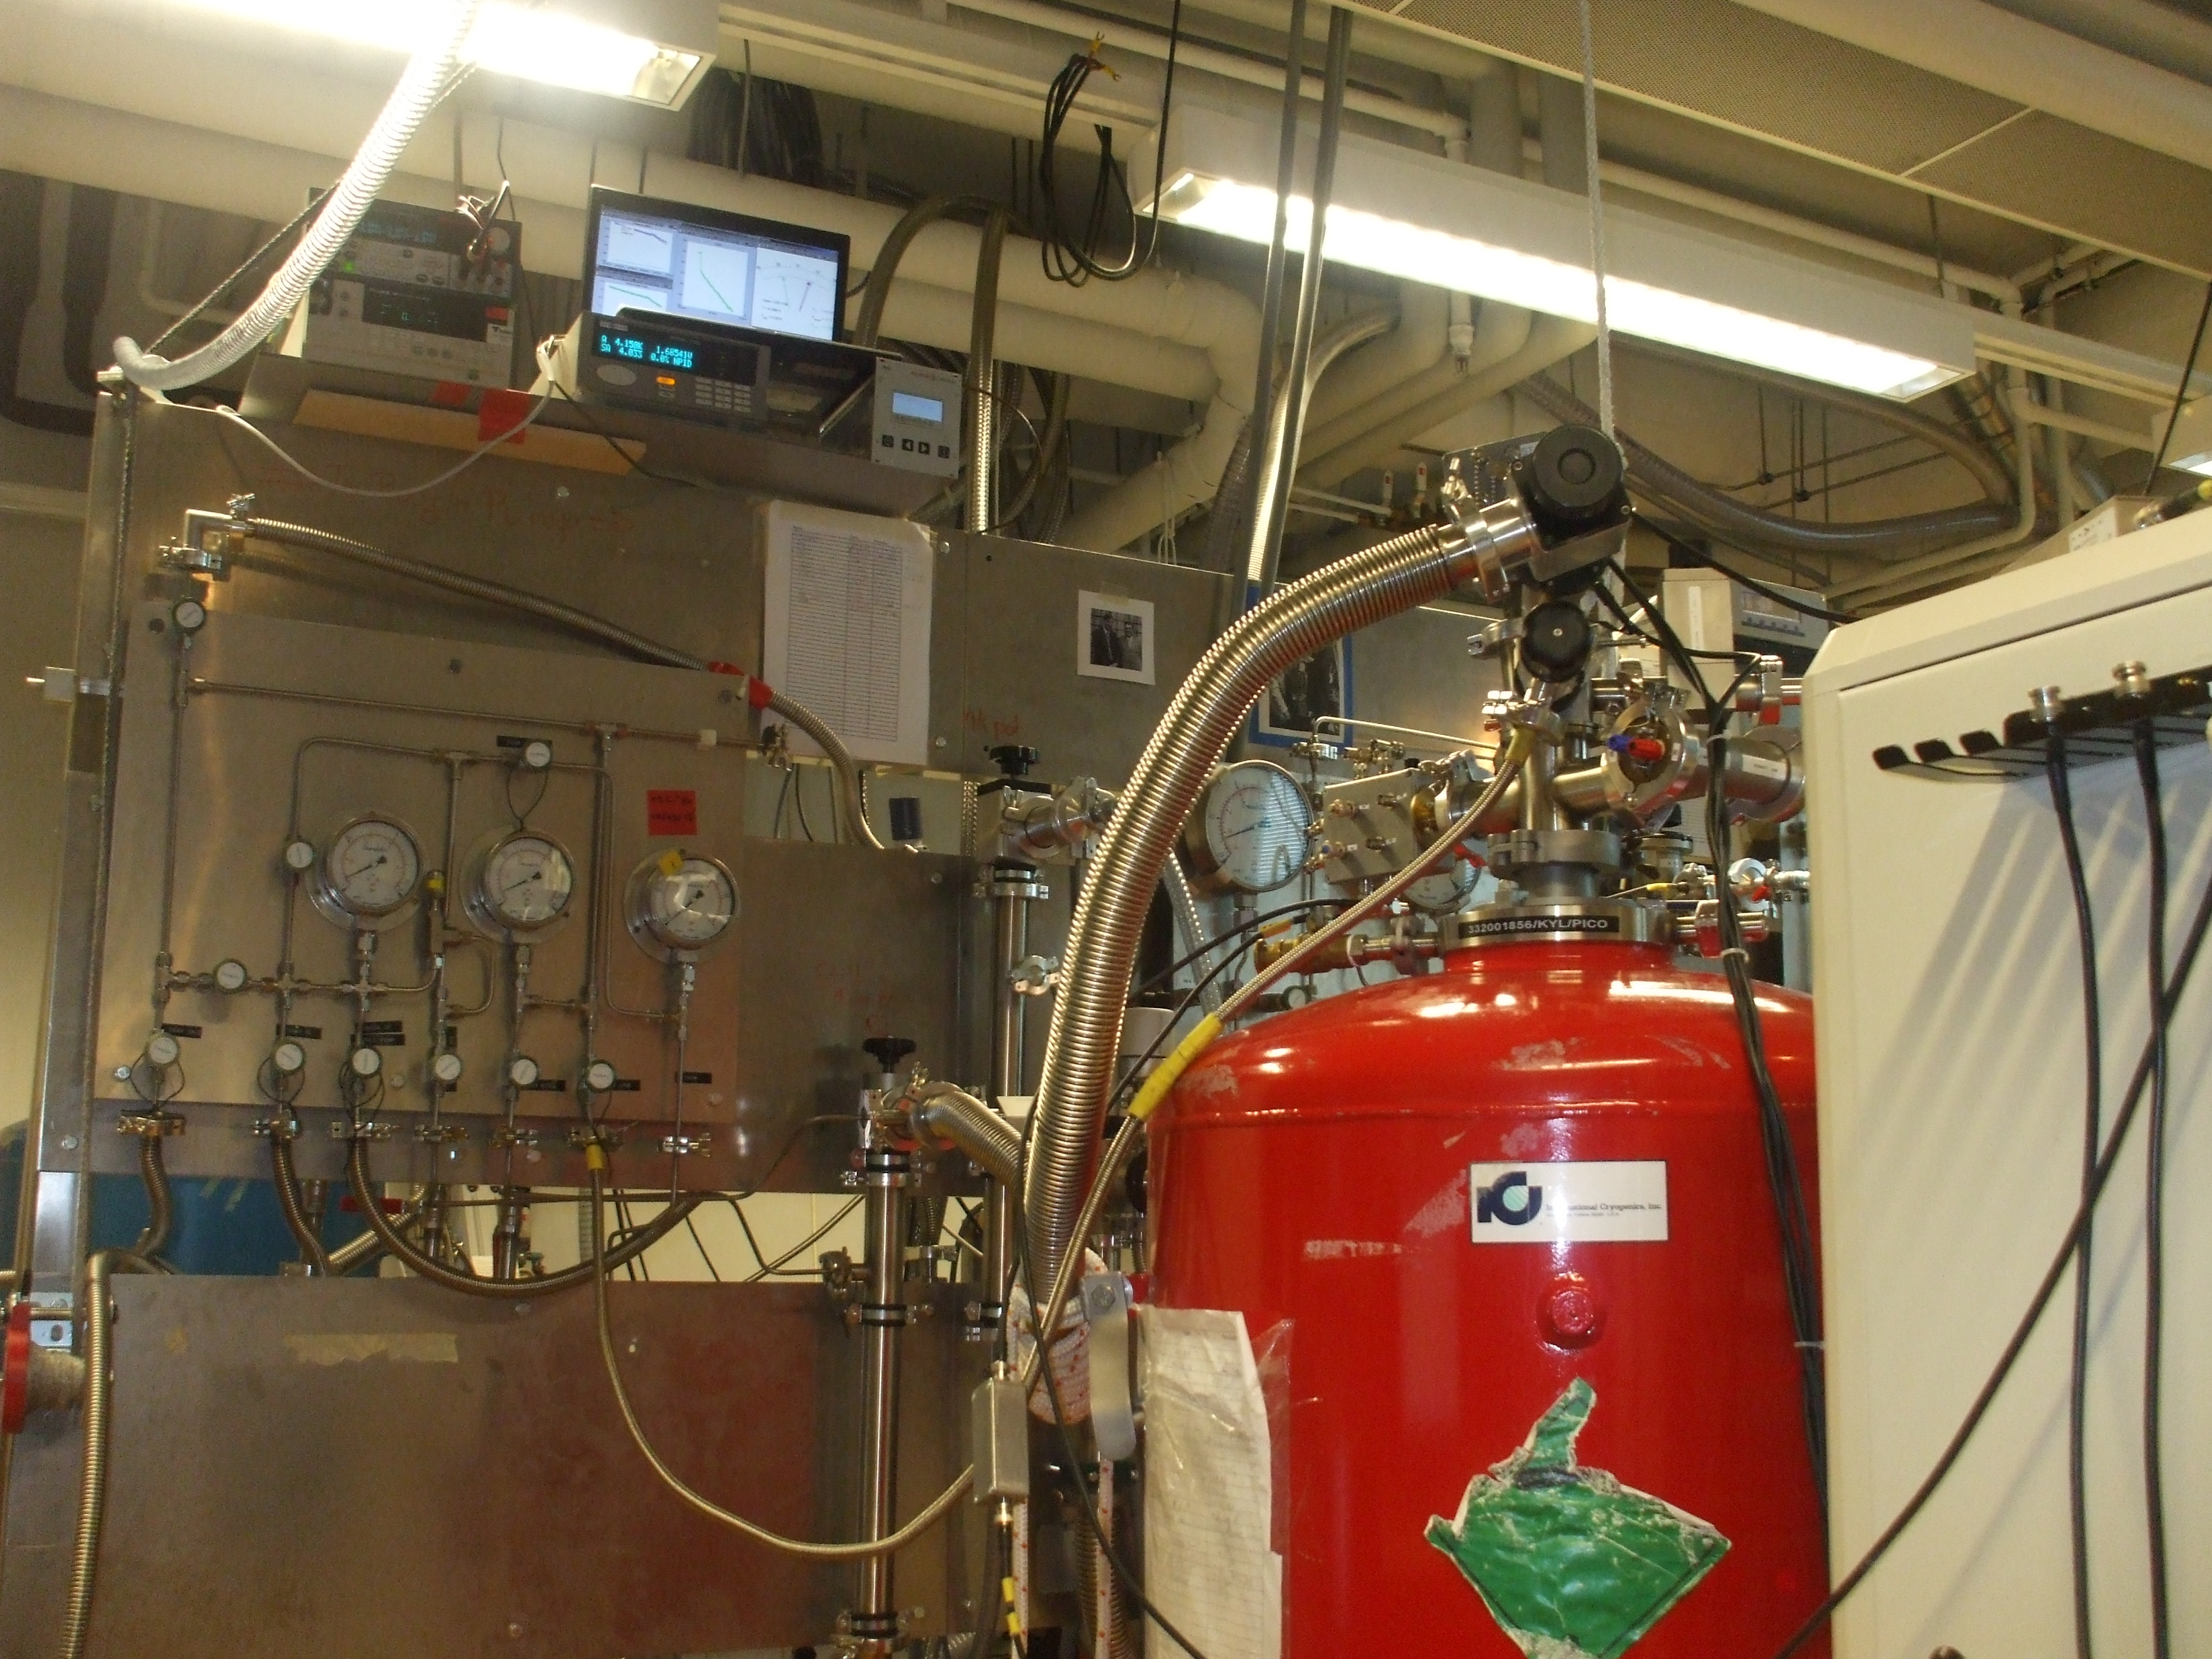
\includegraphics[width=6.4cm]{setup4K.JPG}
                \caption{Picture of the setup when the fridge thermalize at 4.2K}
                \label{Setup4K}
            \end{subfigure}
            \caption{Pictures of the cool down}
            \end{figure}
            
            %After having waited enough, we stop pumping the IVC and we will start to condense. The pressure in the IVC is very low, we stop pumping it and remove the line. We open the 1K pot valves to put some Helium in and pump over it to cool it down to 1K. Since Helium is superfluid at this temperature, we would notice it there was any leak, because it could go everywhere. We put the trap in liquid nitrogen, so that we can flush the condensing and the still lines with mixture. The mixture goes from the pump to the lines through the trap and back to the pump, so it cleans the gas inside the lines : if there was still some air for example. We flush three times to divide the amount of impurities by 10$^8$ (10$^2$ each time). Once the lines are clean, we start to send the mixture to the cryostat through the still line. The still pump contains some mixture, but the tank contains a much larger amount, so we have to open the tank valves to take the mixture from here too. Then we wait until the tak is empty. Once it is empty, and that the temperature is low, we can start to circulate : we close the tank valve and  create a loop for the mixture (See Fig.\ref{loopmixture}), so that it is always moving and cools down the fridge.
            
            \begin{figure}
                \centering
                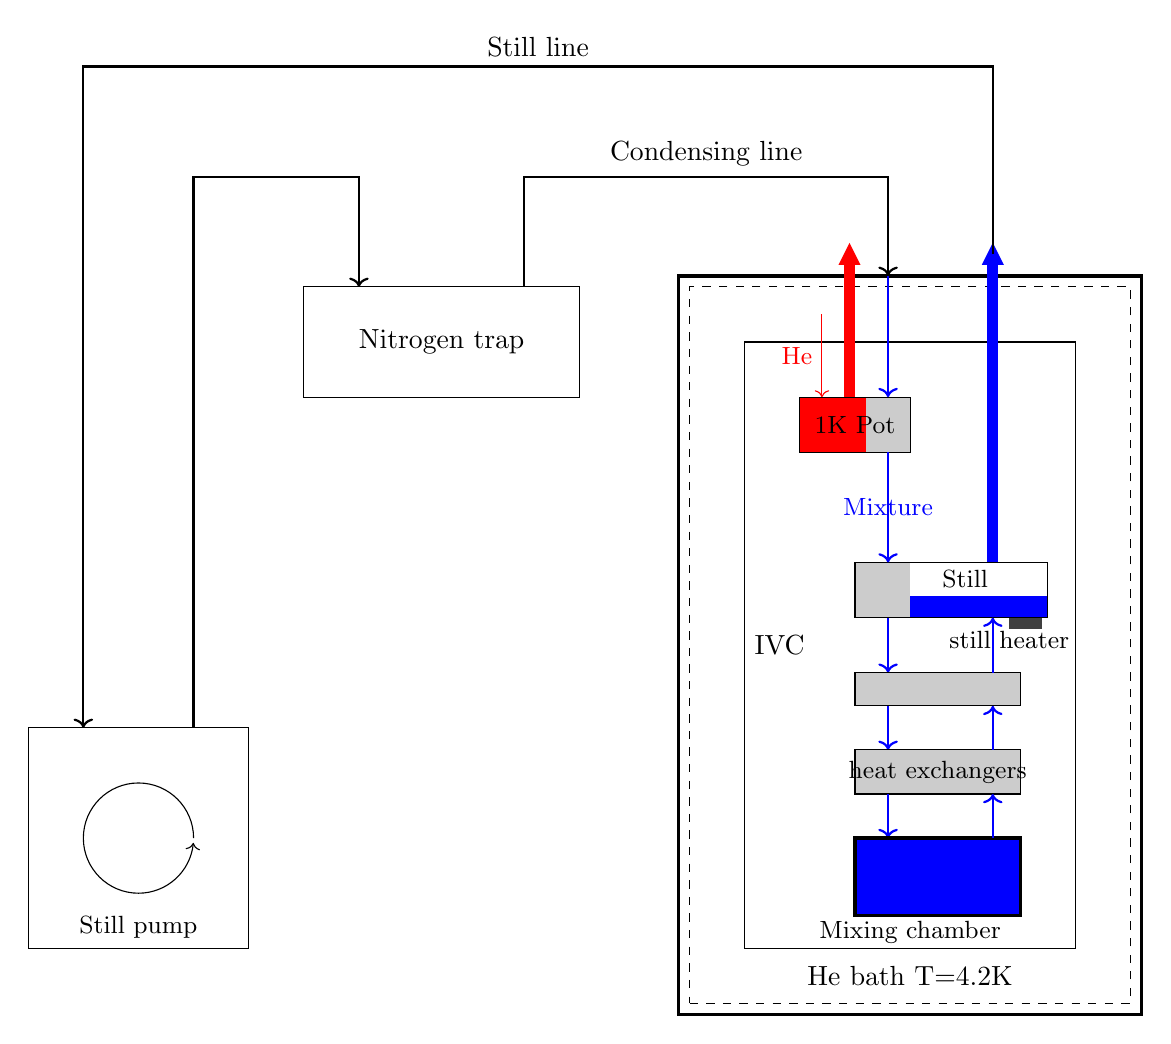
\begin{tikzpicture}[scale=1.4]

\draw (0,2)--(0,4)--(2,4)--(2,2)--cycle;
\draw [->](1.5,3) arc(0:355:0.5);
\draw (1,2)node[above]{{\small Still pump}};

\draw [thick,->](1.5,4)--(1.5,9)--(3,9)--(3,8);
\draw (2.5,8)--(5,8)--(5,7)--(2.5,7)--cycle;
\draw (3.75,7.5)node{Nitrogen trap};
\draw [thick,->] (4.5,8)--(4.5,9)--(7.8,9)node[midway,above]{Condensing line}--(7.8,8.1);

\draw [very thick] (5.9,1.4)--(10.1,1.4)--(10.1,8.1)--(5.9,8.1)--cycle;%HEdewar
\draw (8,1.75)node{He bath T=4.2K};
\draw [dashed] (6,1.5)--(10,1.5)--(10,8)--(6,8)--cycle;
\draw (6.5,2)--(9.5,2)--(9.5,7.5)--(6.5,7.5)--cycle;%IVC
\draw (6.5,4.75)node[right]{IVC};
\fill [color=red] (7,7)--(7.6,7)--(7.6,6.5)--(7,6.5)--cycle;

\draw [color=red,->](7.2,7.75)--(7.2,7)node[midway, left]{{\small He}};
\fill [color=red] (7.4,7)--(7.5,7)--(7.5,8.2)--(7.4,8.2)--cycle;%He
\fill [color=red] (7.35,8.2)--(7.55,8.2)--(7.45,8.4)--cycle;%He
\fill [color=gray!40] (7.6,7)--(7.6,6.5)--(8,6.5)--(8,7)--cycle;%heat exc
\draw (7,7)--(8,7)--(8,6.5)--(7,6.5)--cycle;%1Kpot
\draw (7.5,6.75)node{{\small 1K Pot}};

\draw [color=blue,->, thick](7.8,8.1)--(7.8,7);%mixt
\fill [color=gray!40] (7.5,5.5)--(7.5,5)--(8,5)--(8,5.5)--cycle;
\fill [color=blue] (8,5)--(8,5.2)--(9.25,5.2)--(9.25,5)--cycle;
\draw (7.5,5.5)--(7.5,5)--(9.25,5)--(9.25,5.5)--cycle;%still
\fill [color=gray!150] (8.9,5)--(9.2,5)--(9.2,4.9)--(8.9,4.9)--cycle;
\draw (8.9,4.8)node{{\small still heater}};
\draw [color=blue,->,thick] (7.8,5)--(7.8,4.5); 
\fill [color=gray!40] (7.5,4.5)--(7.5,4.2)--(9,4.2)--(9,4.5)--cycle;

\draw (7.5,4.5)--(7.5,4.2)--(9,4.2)--(9,4.5)--cycle;
\draw [color=blue,->,thick](7.8,4.2)--(7.8,3.8);
\draw (8.5,5.35)node{{\small Still}};
\draw [color=blue,->,thick](7.8,6.5)--(7.8,5.5)node[midway]{{\small Mixture}};%mixt
\fill [color=gray!40] (7.5,3.8)--(7.5,3.4)--(9,3.4)--(9,3.8)--cycle;
\draw (7.5,3.8)--(7.5,3.4)--(9,3.4)--(9,3.8)--cycle;
\draw (8.25,3.6)node{{\small heat exchangers}};
\draw [color=blue,->, thick](7.8,3.4)--(7.8,3);
\fill [color=blue] (7.5,3)--(7.5,2.3)--(9,2.3)--(9,3)--cycle;
\draw [very thick] (7.5,3)--(7.5,2.3)--(9,2.3)--(9,3)--cycle;
\draw (8,2.15)node{{\small Mixing chamber}};
\draw [color=blue,->, thick] (8.75,3)--(8.75,3.4);

\draw [color=blue,->,thick] (8.75,4.5)--(8.75,5);
\draw [color=blue,->,thick] (8.75,3.8)--(8.75,4.2);
\fill [color=blue] (8.7,5.5)--(8.8,5.5)--(8.8,8.2)--(8.7,8.2)--cycle;
\fill [color=blue] (8.65,8.2)--(8.85,8.2)--(8.75,8.4)--cycle;
\draw [->,thick] (8.75,8.3)--(8.75,10)--(0.5,10)node[midway,above]{Still line}--(0.5,4);

\end{tikzpicture}

                \caption[Dilution fridge functioning schematics]{Dilution fridge functioning schematics : The still pump and the nitrogen trap are outside the dewar. The mixture that is injected in the IVC is represented in blue, the $^4$He is in red. The grey parts are heat exchangers}
                \label{loopmixture}
            \end{figure}
            
%             \subsection{Warming up}
%             
%             Warming up the fridge is quite easy, first we have to stop the circulation of the mixture by closing the trap in and start to pump it from both still and condensing lines to the tank, so we open the tank and still valves. The mixture is liquid so it is difficult to pump it in this state. To ease the pumping, we will heat up to evaporate the mixture. For this, there are two lines where we can apply some voltage, which will go through thermoresistor and heat the area and then the mixture. Since the mixture is pump with the still pump, we have to be careful that the pressure does not exceed 1 mbar, or it could damage the pump. To avoid huge augmentation of the pressure we increase slowly the applied voltage, especially around 1.3K when the mixture starts to boil. Of course, we can control the temperature through Matlab, like we did for the cool down. The pressure increases while the mixture is evaporated. It can take one hour until the mixture is totally pumped out.
%             
%             Once it is the case, the temperature increase rapidly and the pressure goes down. Here, we wait five minutes to be sure all the mixture went out. Then, we close all the valves of the condensing line and the still line, we keep pumping the mixture to the tank, finally, we close the tank and remove the fridge from the dewar. Here, the fridge just needs to thermalize at the room temperature, we let it like that for a while before removing the sample and getting the fridge ready for the next cooling.
%             
%             

\chapter{Experimental protocol}
\label{Chap3}

In this part I will focus on the relevant tests made, results of the first tests will be found in Appendix \ref{badtests}.

    \section{Parameters}
    
        The following table describes the different devices used for the realization of the samples and shows the parameters that have to be taken into account during the fabrication. The parameters in bold are the most influent in the results we will obtain, so they are important and the settings needs to be determined precisely.
        
       \vspace{0.5cm}
         
        \begin{tabular}{|c|c|c|}
        \hline
        \textsc{Step}&\textsc{Device}&\textsc{Parameters}\\
        \hline
        Resist deposition&Spinner&Rotation Speed\\
        \hline
        Resist baking&Hot plate&Temperature\\
        \hline
        Pattern design&EBL&\textbf{Dose}, \textbf{Shape(area)}, Resolution\\
        \hline
        Development&MIBK, MG, IPA&\textbf{Duration}\\ 
        \hline
        Deposition of metal&Evaporator&\textbf{Angle}\\
        \hline
        Oxidation&Evaporator&\textbf{Pressure}, \textbf{Duration}\\
        \hline
        Plasma Etching&Plasma gun&\textbf{Duration}, Position\\
        \hline
        Lift-off&Aceton&$\varnothing$ \\
        \hline
        \end{tabular}
        
        \vspace{0.5cm}
        
            
            The chip we realize consists in twenty samples, with four different surface areas (0.5, 1, 1.5 \& 2 $\mu m^2$) and five different electron doses (from 2000 to 3000 by 250 $c/\mu m^2$) in the EBL. This gives us some statistics : we do not stick to one result but we have several ones to make sure the datas we get are relevant and not due to any problem. Moreover, some little troubles can always occur on one of the samples (EBL default, speck of dust...) and fabricating 20 of them avoids to loose a whole attempt. Mathieu already defined some settings such as the development time and he made the patterns and the EBL writing.
                        
        \section{Experimental procedure}
        
            In order to have coherent results I have always followed the same process to realize the samples. Based on 4 layers of MMA and one layer of PMMA and EBL dose from 2000 to 3000 $\mu m^2$, according to the pattern in Fig. \ref{patternjunction}, I develop 20s in MIBK, 20s in MG and IPA. Then I evaporate 20nm of Al. Depending on the sample I want to make, I can strongly oxidize with a pressure of 200mbar of O$_2$ during 10 min. Then, I can use the plasma to etch, the parameters are a pressure of $4.10^{-4}mbar$ of Argon, a power of 40mA, an extraction voltage of -0.8kV (lowered down to -250V in July, due to problems that high voltage caused) and a Ion Energy of 1.5kV. I can also oxidize with a pressure of 2mbar during 2min. Finally, I evaporate 25nm of Cu before letting the sample in lift-off for more than an hour..
            
            I have realized samples with strong oxidation and plasma etching to see how much oxide was etched, then I have realized samples with strong oxidation, plasma etching and regular oxidation and regular oxidation reference samples in order to cool them down to see the differences and so the effect of the plasma on the quality of the NIS junction.  You can find an exhaustive table of the parameters used for each test in Appendix \ref{parametertable}
            
            \begin{figure}
                \centering
                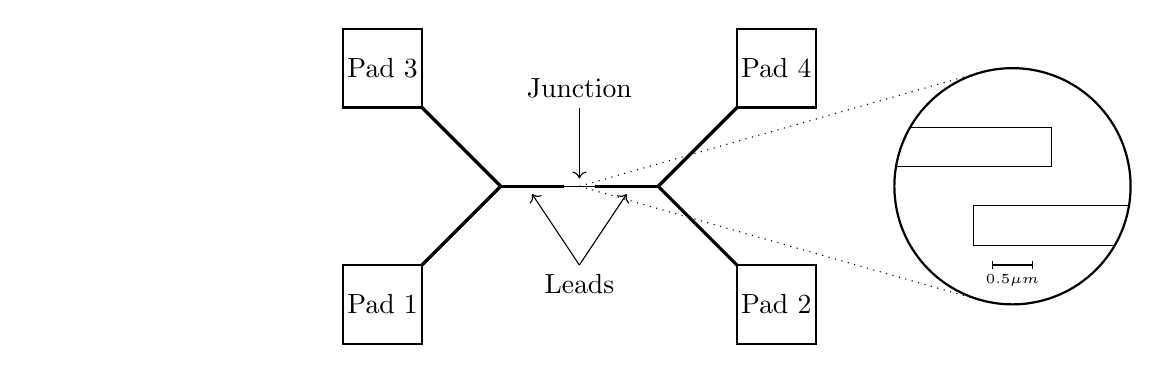
\begin{tikzpicture}
                    \draw [thick](0,0)--++(1,0)--++(0,1)--++(-1,0)--cycle;
                    \draw [thick](0,3)--++(1,0)--++(0,1)--++(-1,0)--cycle;
                    \draw [thick](5,0)--++(1,0)--++(0,1)--++(-1,0)--cycle;
                    \draw [thick](5,3)--++(1,0)--++(0,1)--++(-1,0)--cycle;
                    \draw [very thick](1,1)--(2,2);
                    \draw [very thick](1,3)--(2,2);
                    \draw [very thick](5,1)--(4,2);
                    \draw [very thick](5,3)--(4,2);
                    \draw [very thick](2,2)--(2.8,2);
                    \draw [very thick](4,2)--(3.2,2);
                    \draw (2.8,2)--(3.2,2);
                    \draw [->] (3,3)--(3,2.1);
                    \draw (3,3)node[above]{Junction};
                    \draw (0.5,0.5)node{Pad 1};
                    \draw (0.5,3.5) node{Pad 3};
                    \draw (5.5,0.5)node{Pad 2};
                    \draw (5.5,3.5)node{Pad 4};
                    \draw [->] (3,1)--(2.4,1.9);
                    \draw [->] (3,1)--(3.6,1.9);
                    \draw (3,1)node[below]{Leads};
                    \draw [dotted,thin] (3,2)--(8.1,3.45);
                    \draw [dotted,thin] (3,2)--(8.1,0.55);
                    \draw [thick](8.5,2) circle(1.5);
                    \draw (7.2,2.75)--(9,2.75)--(9,2.25)--(7.02,2.25);
                    \draw (9.8,1.25)--(8,1.25)--(8,1.75)--(9.98,1.75);
                    \draw (8.25,1.05)--(8.25,0.95);
                    \draw (8.75,1.05)--(8.75,0.95);
                    \draw (8.25,1)--(8.75,1)node[midway, below]{\tiny{0.5$\mu m$}};
                    \draw [color=white](-4,2)--(-4,2.01);
                \end{tikzpicture}
                \caption{Pattern of the junctions}
                \label{patternjunction}
            \end{figure}
            
            \section{Problems with the devices}
            
            When I was here, there have been some problems with the evaporator LISA which I used to make the structures. The plasma gun seemed to have a problem in the begining of July, since it didn't work properly. We could see that nothing happened when we set the power current. It was cleaned and repaired and the main user advised to limit the Extraction to -250V to avoid future breakdown. After this, the plasma seemed to act differently, it seemed more powerful according to the results (See \ref{Chap4}). Then, just before I left, everyone seemed to have troubles with the junctions made in the evaporator. I tried to 
            
            \section{Measurement setup}
            \subsection{Room temperature setup}
            
            We first used a method to measure the samples but it was not rigorous enough, I talk about it in Appendix \ref{badmeasures}.
                
                Let's focus on the good measurements. I have made four-probe resistance measurements on the samples I have fabricated with a probe station. The four-probe measurements make sense as it is the only way to measure the real resistance of the device, without parasite resistances. The probestation make a slope of voltage from -100 mV to 100 mV, measure the voltage and the current between two electrodes and trace an I-V curve. It export the data obtained in .DAT files with the current and voltage tables. I have then realized a Matlab program to exploit them efficiently and be able to trace charts showing the more parameter dependances possible.
                
            \subsection{Low temperature setup}
                
                Since the samples I make are superconductors-based structures, it is worth measuring them at low temperature to have the superconductivity state of Al. The critical temperature of Al is 1.2K, so we have to cool the sample lower than this temperature to obtain results. We use a dilution cryostat as the ones described earlier. Once the sample is cold, we can start the measurements.
                
                There are devices that can be connected to the cryostat lines wich are lined to the samples. Everything is controlled through Matlab programs. I have adapted an existing program to make it fit better with the measurements I wanted to do and the way I wanted to exploit the datas. First, I have to set the parameters, then the program is linked with the devices, it controls the generator to make a voltage slope and in the meanwhile it asks the multiplexer to get the bias voltage and the voltage which comes from the current amplifier (See Fig.\ref{circuit}). These are rough values that are not the real ones. I can draw IV curves to check that everything is correct : good $V_bias$ range, accurate current amplification... Then the program saves the datas that I will exploit with a better program later. The program I wrote allows to draw the IV curves, and determine easily the resistance and the leakage of the junctions.
                                
        \begin{figure}
            \centering
            \begin{circuitikz}
                \draw 
            (0,0) node[ground]{} 
                to [V,v=$DC$,v_>=$V_{meas}$] (0,3)
                to [R=5<\kilo\ohm>] (3,3)
                to [R=20<\ohm>,*-,v_<=$V_{bias}$] (3,0)
                node[ground] {}
            (3,3) to [R=$R_{sample}$,i=$i_{sample}$] (8,3)
                to [ammeter, v^<=$V->I_{amplifed}$] (8,0) node[ground] {}
            ;
            \end{circuitikz}
            \caption{Schematics of the set up for low temperature measurements}
         \label{circuit}
        \end{figure}
        
                
                
                
                
                
                
            

\pagestyle{fancy}

\chapter{Results and discussions}
\label{Chap4}

This part will present the results the measurements gave and the discussions we can have give according to these results.

\section{Room Temperature Results}
                \subsection{Reference Samples}
                
                Every experiment needs references to rely on. Before starting anything with the plasma, it is important to know the behaviour of the same structures (in terms of parameters) without plasma, to have access to a comparison. The three reference samples are a clean contact (Al/Cu), a strong oxidation reference (as a native oxidation imitation) (Al/Al Oxide/Cu) and a tunnel junction (Al/Al Oxide/Cu).
                
                The first junction is a clean contact with only Al and Cu as a reference. Since the contact is clean, the resistance of the interface between the two metals should be negligible, then the resistance we measure is :
                
                \begin{equation}
                  R=\sum_{Al,Cu}\dfrac{\rho L}{S}  
                  \label{loidohm}
                \end{equation}
                
                The resistance does not depends on the surface area of the junction, as you can see in Fig. \ref{cleancontact} the results of four probes measurements. As expected the resistance does not depend on the resistance of the surface of the junction.
                The theoretical calculus from this law with the parameters used gives $78\Omega$, which is close to the value we find. There are some uncertainties : the thickness of the metal is not very precise, the dimensions of the device can differ a bit from the pattern dimension. However, the order of magnitude is correct, so our reference for the leads resistance is around $70\Omega$.

                
                \begin{figure}
                    \centering
                    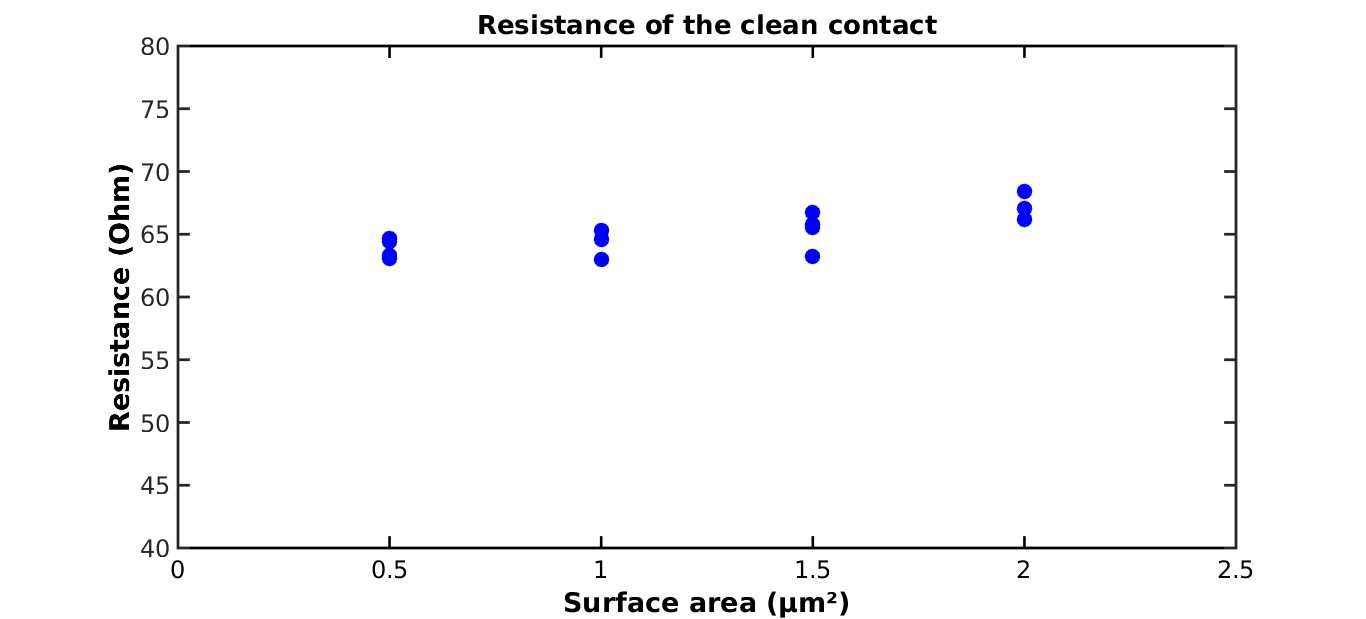
\includegraphics[width=15cm]{Rclean.png}
                    \caption{Resistance of clean contact in function of the surface area}
                    \label{cleancontact}
                \end{figure}
                
           
                After the clean contact, the second reference sample is with a strong oxidation (10 min at an oxygen atmosphere of 200mbar).

                For the NIS junctions, it is more relevant to draw conductance in function of the surface area of the junction. Indeed, the previous law (Eq. \ref{loidohm}) is correct for an insulator, except that $\rho_{AlOx}$ is order of magnitudes higher than $\rho_{Al}$ or $\rho_{Cu}$ and the surface of the junction is the surface of the insulator considered. The resistance of the device is mostly the resistance of the junction, and the conductance of the junction is linear with the surface. The measurements on these samples gave the conductance curve represented in Fig. \ref{Strongox} where :
                \[\dfrac{1}{R}\propto S\]
                
                We can extract a parameter from the slope :
                
                \[RS=7.18k\Omega.\mu m^2\]
                
                This parameter is linked with the thickness of the oxide layer.
                                
                \begin{figure}
                    \centering
                    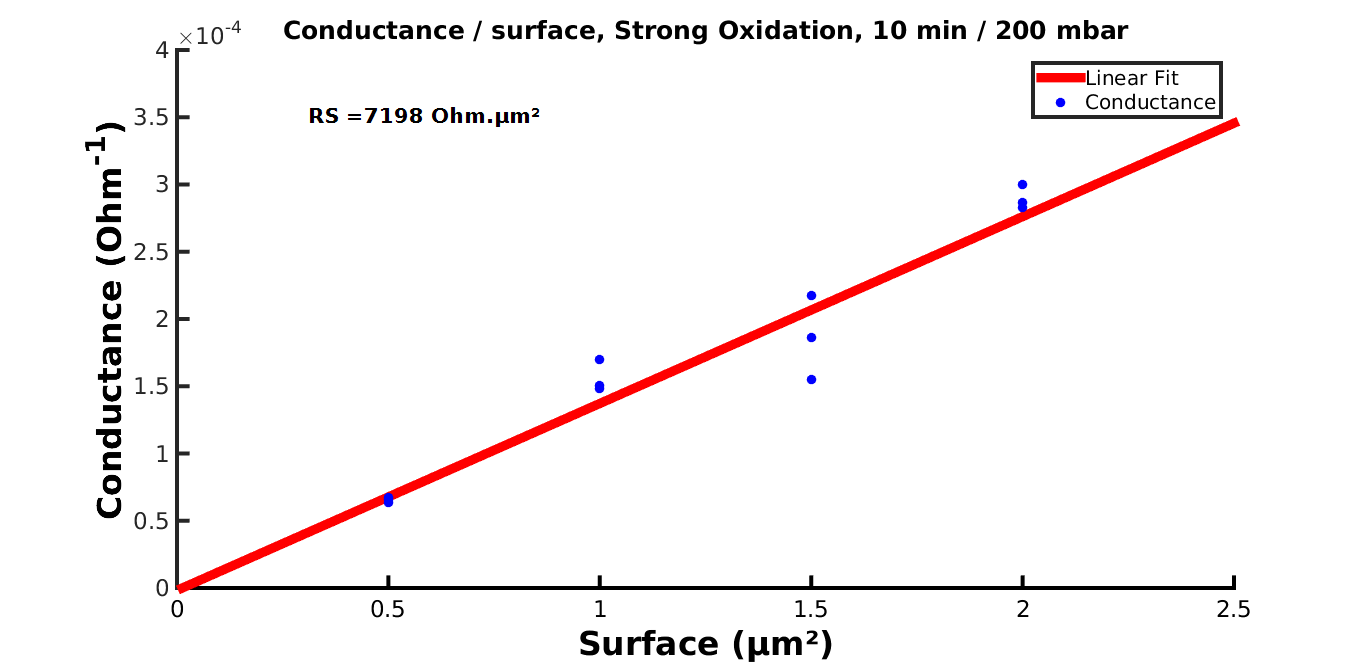
\includegraphics[width=15cm]{ConductanceFitStrongOx.png}
                    \caption{Conductance in function of surface area for a strong oxidized sample}
                    \label{Strongox}
                \end{figure}
                
                In order to cover a large range of resistance, the third reference sample is also a tunnel junction but lighter than the previous one (2min at an oxygen atmosphere of 2mbar).
                
                Again, it is more relevant to draw the conductance (See Fig. \ref{Regularox}) to determine the RS parameter.
                
                \begin{figure}
                    \centering
                    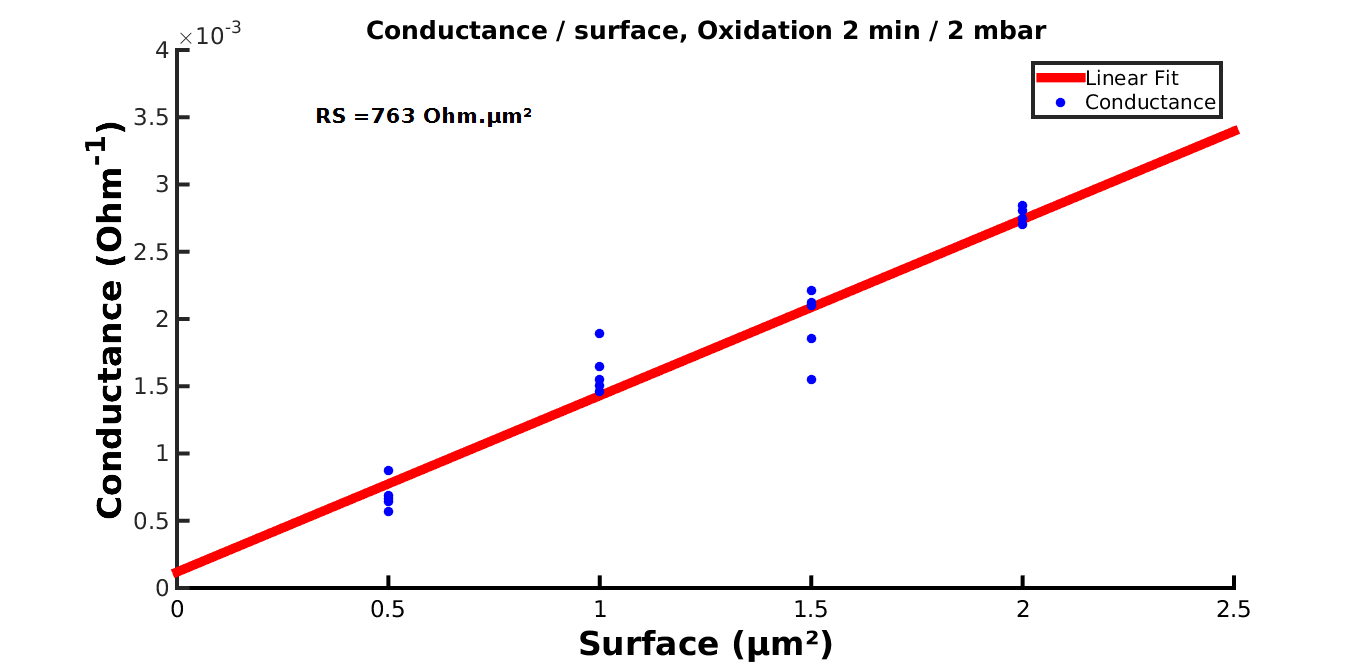
\includegraphics[width=15cm]{ConductanceFitOx.png}
                    \caption{Conductance in function of surface area for a tunnel junction sample}
                    \label{Regularox}
                \end{figure}
                                
                \[RS=763\Omega.\mu m^2\]
                
                RS is ten times less important than for the strong oxidation. It means that the oxide layer is quite thinner in this case, which is normal since the Al was less oxidized in this case.
                These three references give us a base to evaluate the quantity of oxide we etch when we use the plasma.
                \subsection{Plasma Etching : Position of the sample}
                
                The first test to do with the plasma etching is to determine if the beam is focused on the whole sample stage (15cm diameter) and not only on the center. This information will ensure a good homogeneity of the etching on all the surface. In order to do so, four samples where placed on the sample holder : one in the center and three on the side (see inset of Fig. \ref{PlasmaPosition}). The layer of evaporated Al was strongly oxidized, then the oxidation layer was etched by argon plasma for 10 min. Finally, we have made a clean contact by evaporating Cu. The Figure \ref{PlasmaPosition} shows the results of these tests. We can see that the position does not affect the resistance of the sample so we can assume that the etching is quite uniform. And another conclusion of this graphe is that 10 min of plasma are enough to etch all the Al oxide : there is no surface dependance like for the oxidized samples and the resistance is about the same order of magnitude than the clean contact junction. The value is a bit higher because the plasma etches the oxide, so the Al layer is thinner (since AlOx is not deposed on top of Al), which reduce the surface section of the lead, thus, it increases the resistance.
              
                \begin{figure}
                    \centering
                    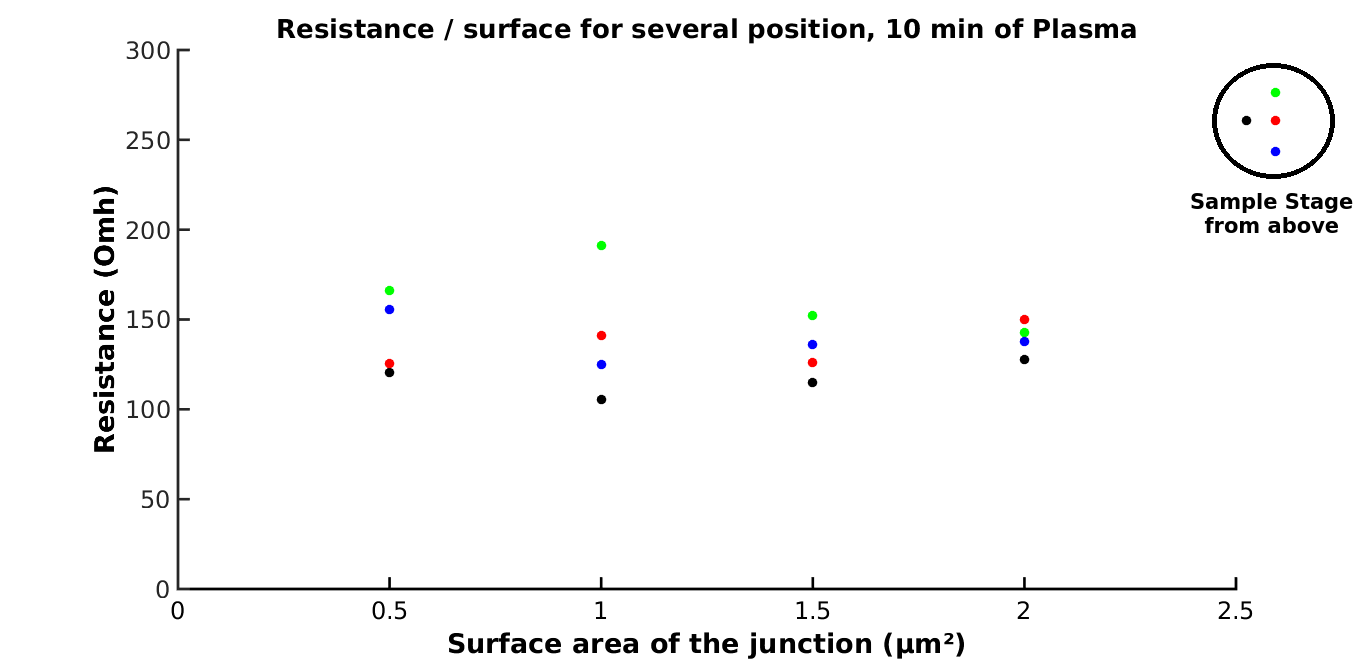
\includegraphics[width=15cm]{R_Position.png}
                    \caption{Resistance in function of surface for different positions of the samples on the LISA's sample stage}
                    \label{PlasmaPosition}
                \end{figure}               
                
                
                \subsection{Time of plasma etching}
                
                The time during which the sample is exposed to the plasma is important and determine how much materials will be etched and implicitely the resistance of the sample. The process is the same for all the samples, only the etching duration is modified.
                The Figure \ref{PlasmaTimeBefore} shows the resistance compared to plasma etching duration before the cleaning of the plasma gun. We can see that there is not a lot of differences between 10 and 20 minutes but the most relevant result is what we can see on the Figure \ref{PlasmaTimeAfter}, with samples made after the cleaning, it seems that less than 5 minutes are enough to etch all the oxide, since the results are very similar, yet for totally different duration times. It means that the cleaning had an effect on the plasma behavior.
                \begin{figure}
                    \centering
                    \begin{subfigure}[t]{0.99\textwidth}
                    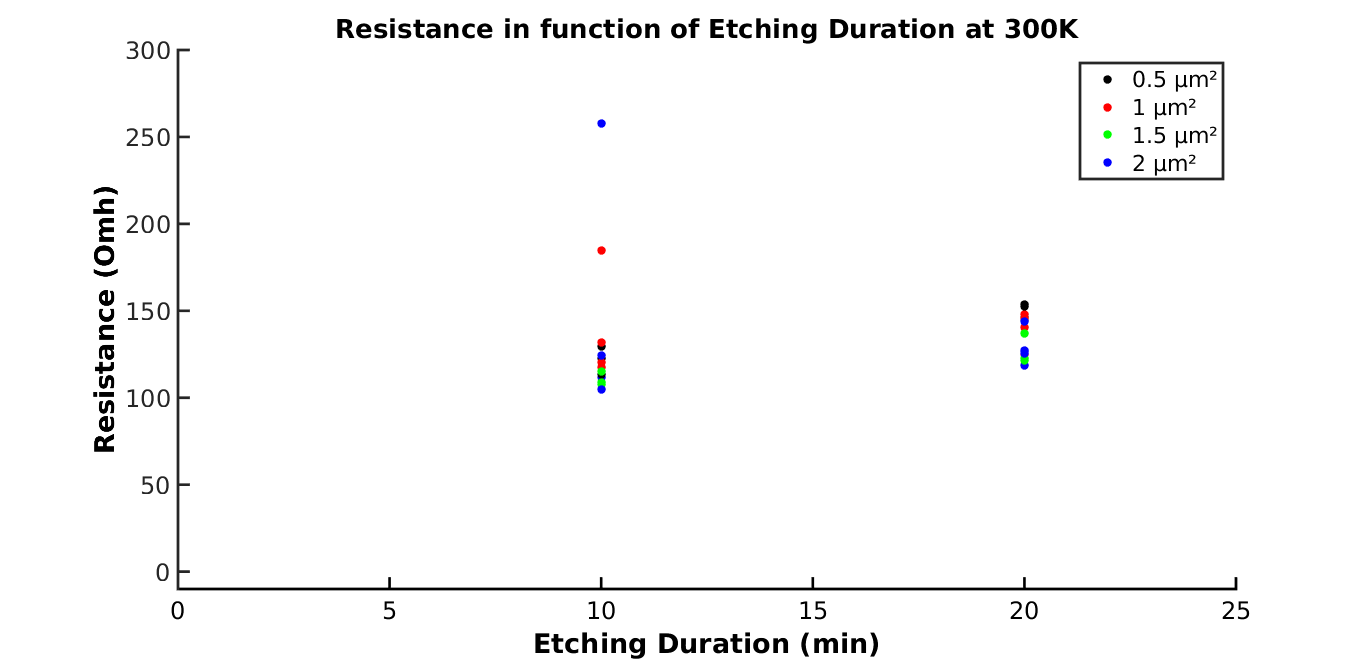
\includegraphics[width=14.9cm]{R_TimeBefore.png}
                    \caption{Resistance in function of Plasma Etching duration before the cleaning}
                    \label{PlasmaTimeBefore}
                    \end{subfigure}
                    ~
                    \begin{subfigure}[t]{0.99\textwidth}
                    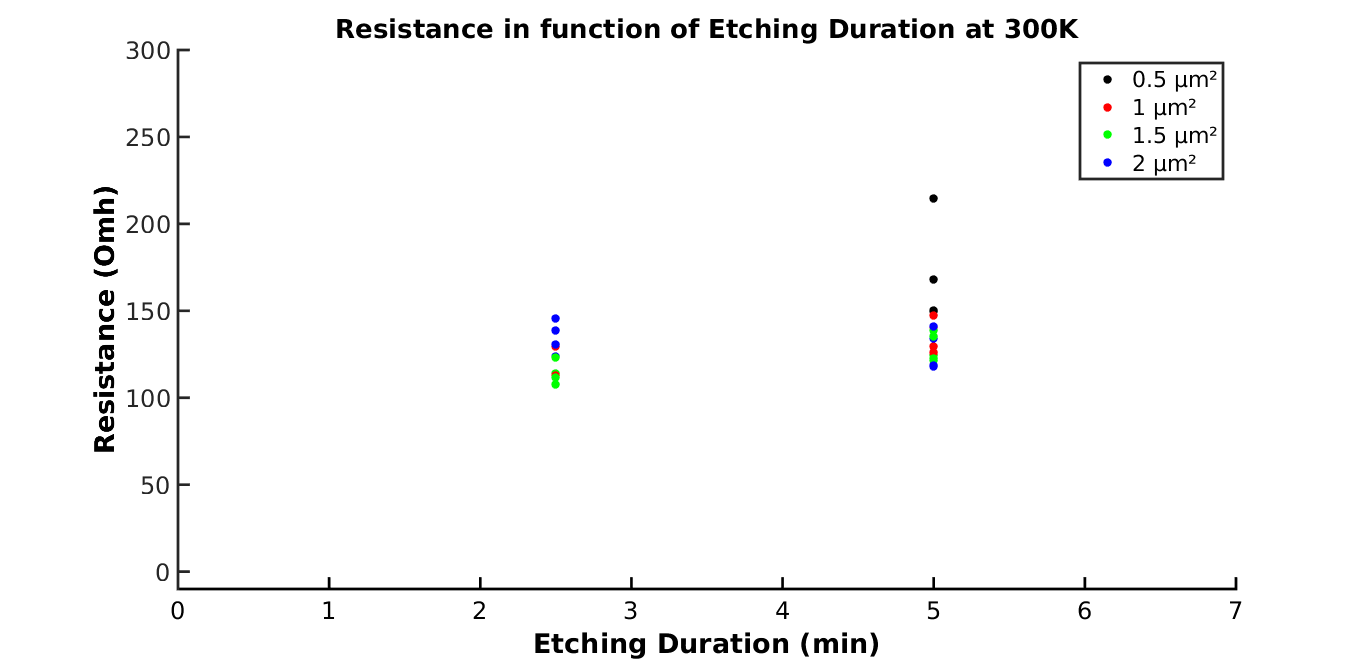
\includegraphics[width=14.9cm]{R_TimeAfter.png}
                    \caption{Resistance in function of Plasma Etching duration after the cleaning}
                    \label{PlasmaTimeAfter}
                    \end{subfigure}
                \end{figure}
                
            \subsection{Wafer Etching}
                According to the previous results, we can think that the oxygen cleaning made the plasma gun more powerful. Here is an observation that confirms this. The Figure \ref{WaferEtch} shows a SEM image of a sample exposed 10 minutes under the plasma after the oxygen cleaning. We can see that the plasma created a hole in the wafer, before the deposition of the copper above it.
                
            \begin{figure}
                \centering
                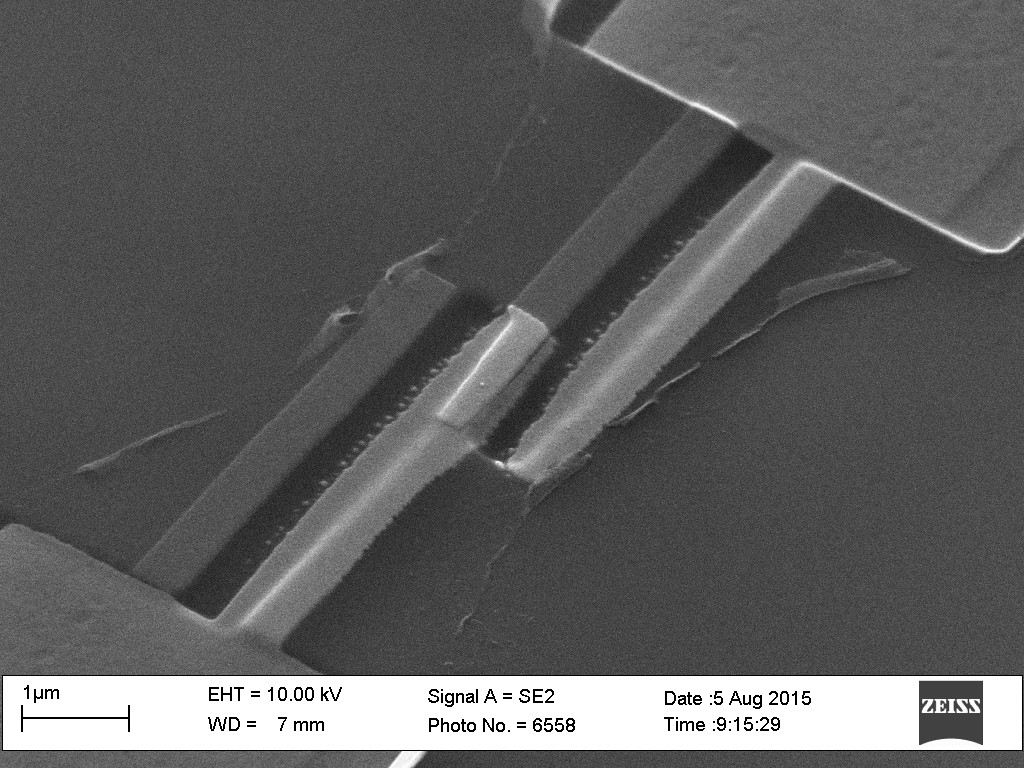
\includegraphics[width=250pt]{tiltSEM.jpg}
                \caption{SEM Image of a sample where the wafer was etched by plasma}
                \label{WaferEtch}
            \end{figure}
                
                \section{Low temperature measurements}
                
                \subsection{NIS Junction}
                
                The Figure \ref{IVlargeNIS} shows the I-V curve that was obtained at low temperature. The curve correspond to what the theory predicts. At a large range of $V_{bias}$ we see almost a strait line : there is tunneling when $V_{bias}$ goes over or under the threshold that the energy gap represents and a flat part in the middle when $V_{bias}$ does not reach the threshold. At a lower range of $V_{bias}$, closer to the limits of the tunneling, we can see (Fig. \ref{IVleakNIS}) better that the flat part is not constant : there is a leakage current, yet the slope is orders of magnitude below the tunneling current. But, there is another phenomenon visible : inside the leakage current there is a part that is steeper, which is the Andreev current, another transport phenomenon \cite{Andreev}.
                
                 The relation between the tunneling current and the leakage current is about 10$^{-4}$ which is quite good. These results are reproducible between different runs and samples. 
                
                \begin{figure}
                    \centering
                    \begin{subfigure}{\textwidth}
                    \centering
                    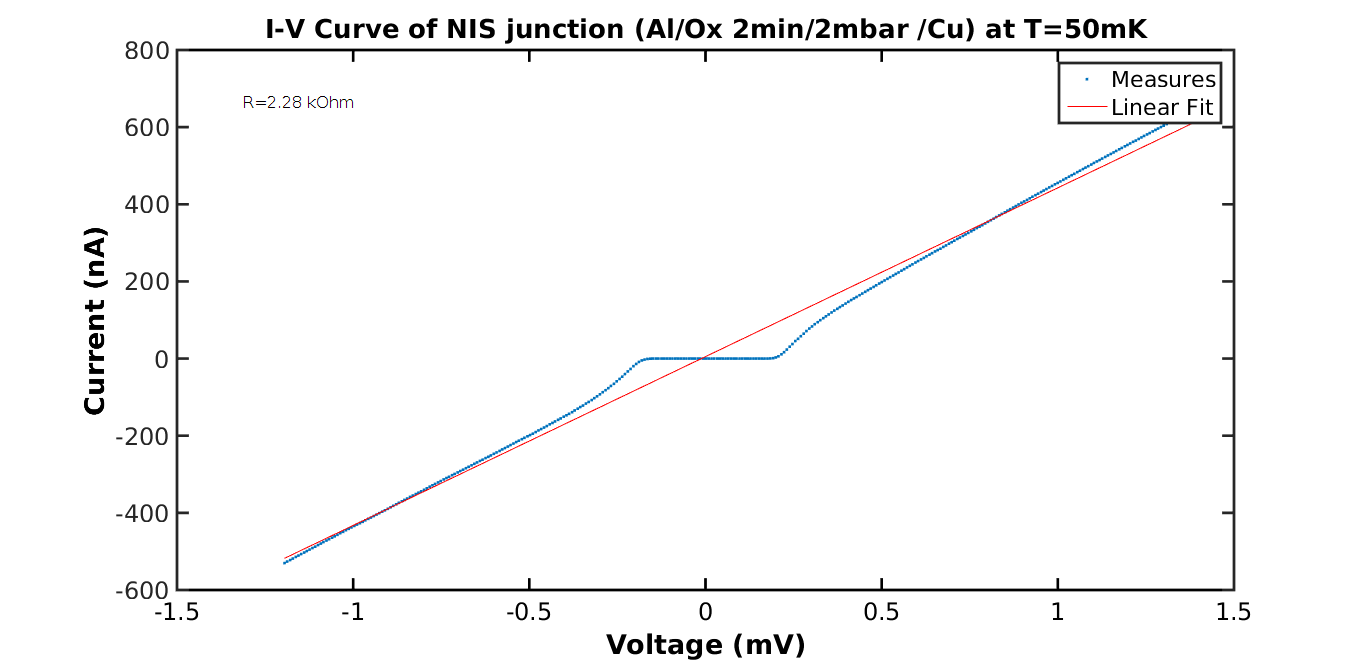
\includegraphics[width=15cm]{IVlargeNIS.png}
                    \caption{IV curve of NIS junctions with an oxidation under a pressure of 2mbar of O$_2$ during 2 minutes at 50mK}
                    
                    \label{IVlargeNIS}
                    \end{subfigure}
                    ~
                    \begin{subfigure}{\textwidth}
                    \centering
                    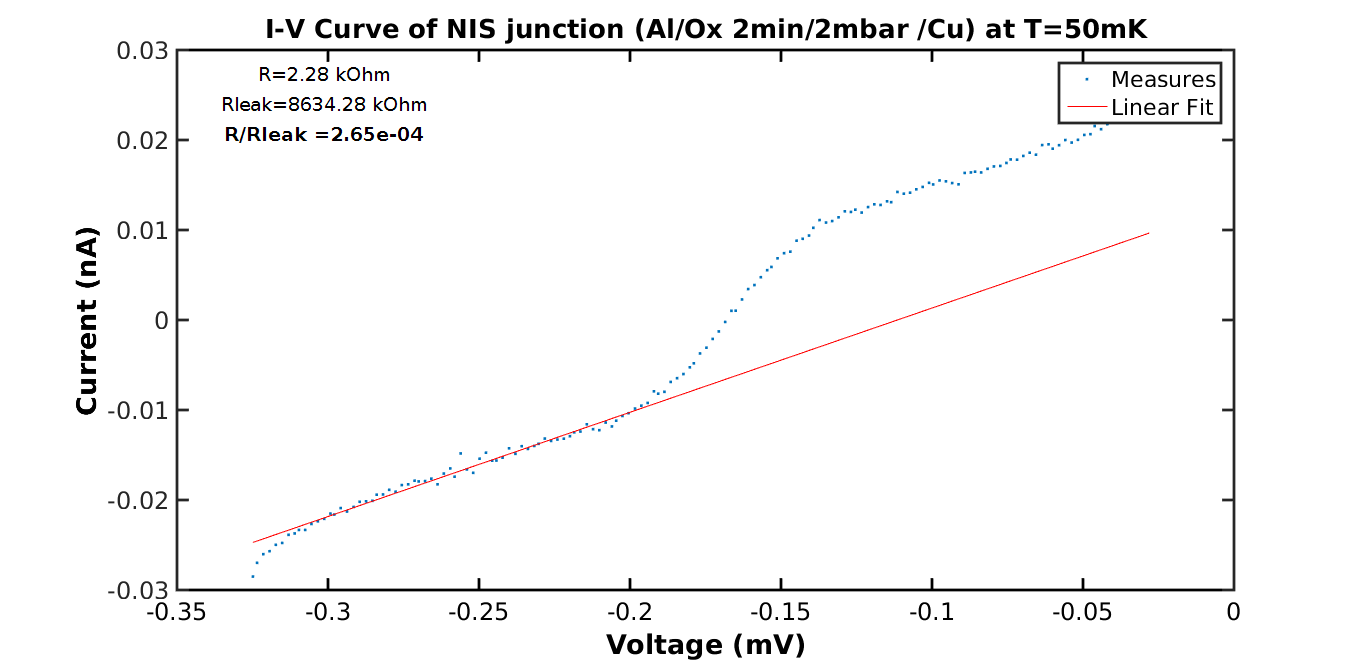
\includegraphics[width=15cm]{IVleakNIS.png}
                    \caption{Zoom in IV curve of NIS junctions with an oxidation under a pressure of 2mbar of O$_2$ during 2 minutes at 50mK}
                    \label{IVleakNIS}
                    \end{subfigure}
                \end{figure}
        
                Moreover, according to the theory, since the tunneling current is based on the density of states of the two material, if the temperature is modified, the current should be modified. Thermal agitation will have some effects on the I-V curves of the NIS junctions. Indeed, as we can see in Fig. \ref{Tsweep}, the coldest the junction is, the sharper the edges are. Heating will bring electrons in states above the Fermi level, and they will be able to tunnel, even if $|eV|<\Delta$.
                
                \begin{figure}
                    \centering
                    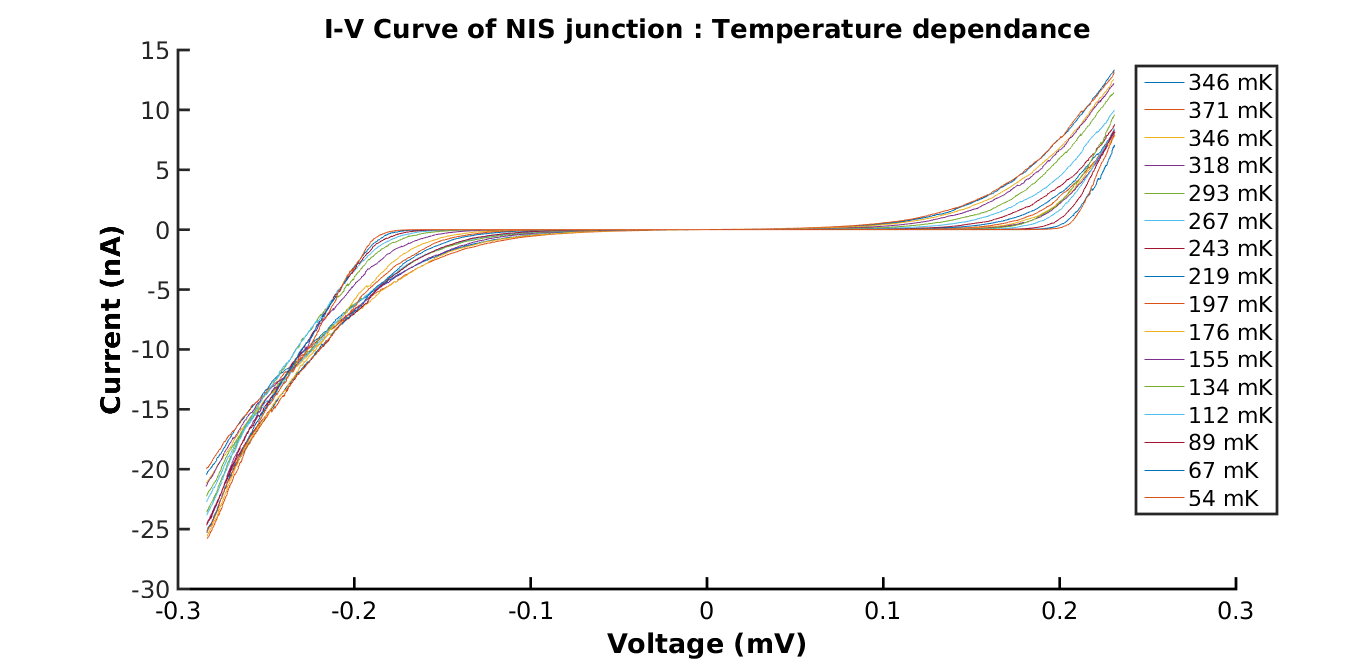
\includegraphics[width=15cm]{Tsweep.png}
                    \caption{Evolution of the IV curves of a NIS junction with the temperature}
                    \label{Tsweep}
                \end{figure}
                
                      
                \subsection{Plasma etched samples}
                This part shows the results of the samples where Al was strongly oxidize, then plasma etched and oxidized again to make a tunnel barrier. In order to discriminate the quality of the junctions by themselves, a reference sample was always done at the same time (without plasma etching and with tunnel barrier). Indeed, the junctions can be bad due to external reasons (polluted chamber, bad materials).
                The Figure \ref{PlasmaOx} shows the IV curves which were obtained for a plasma etched sample and the Figure \ref{ReferenceOx} show the correspondant regular oxidation reference for this sample.
         
        \begin{figure}
            \centering
            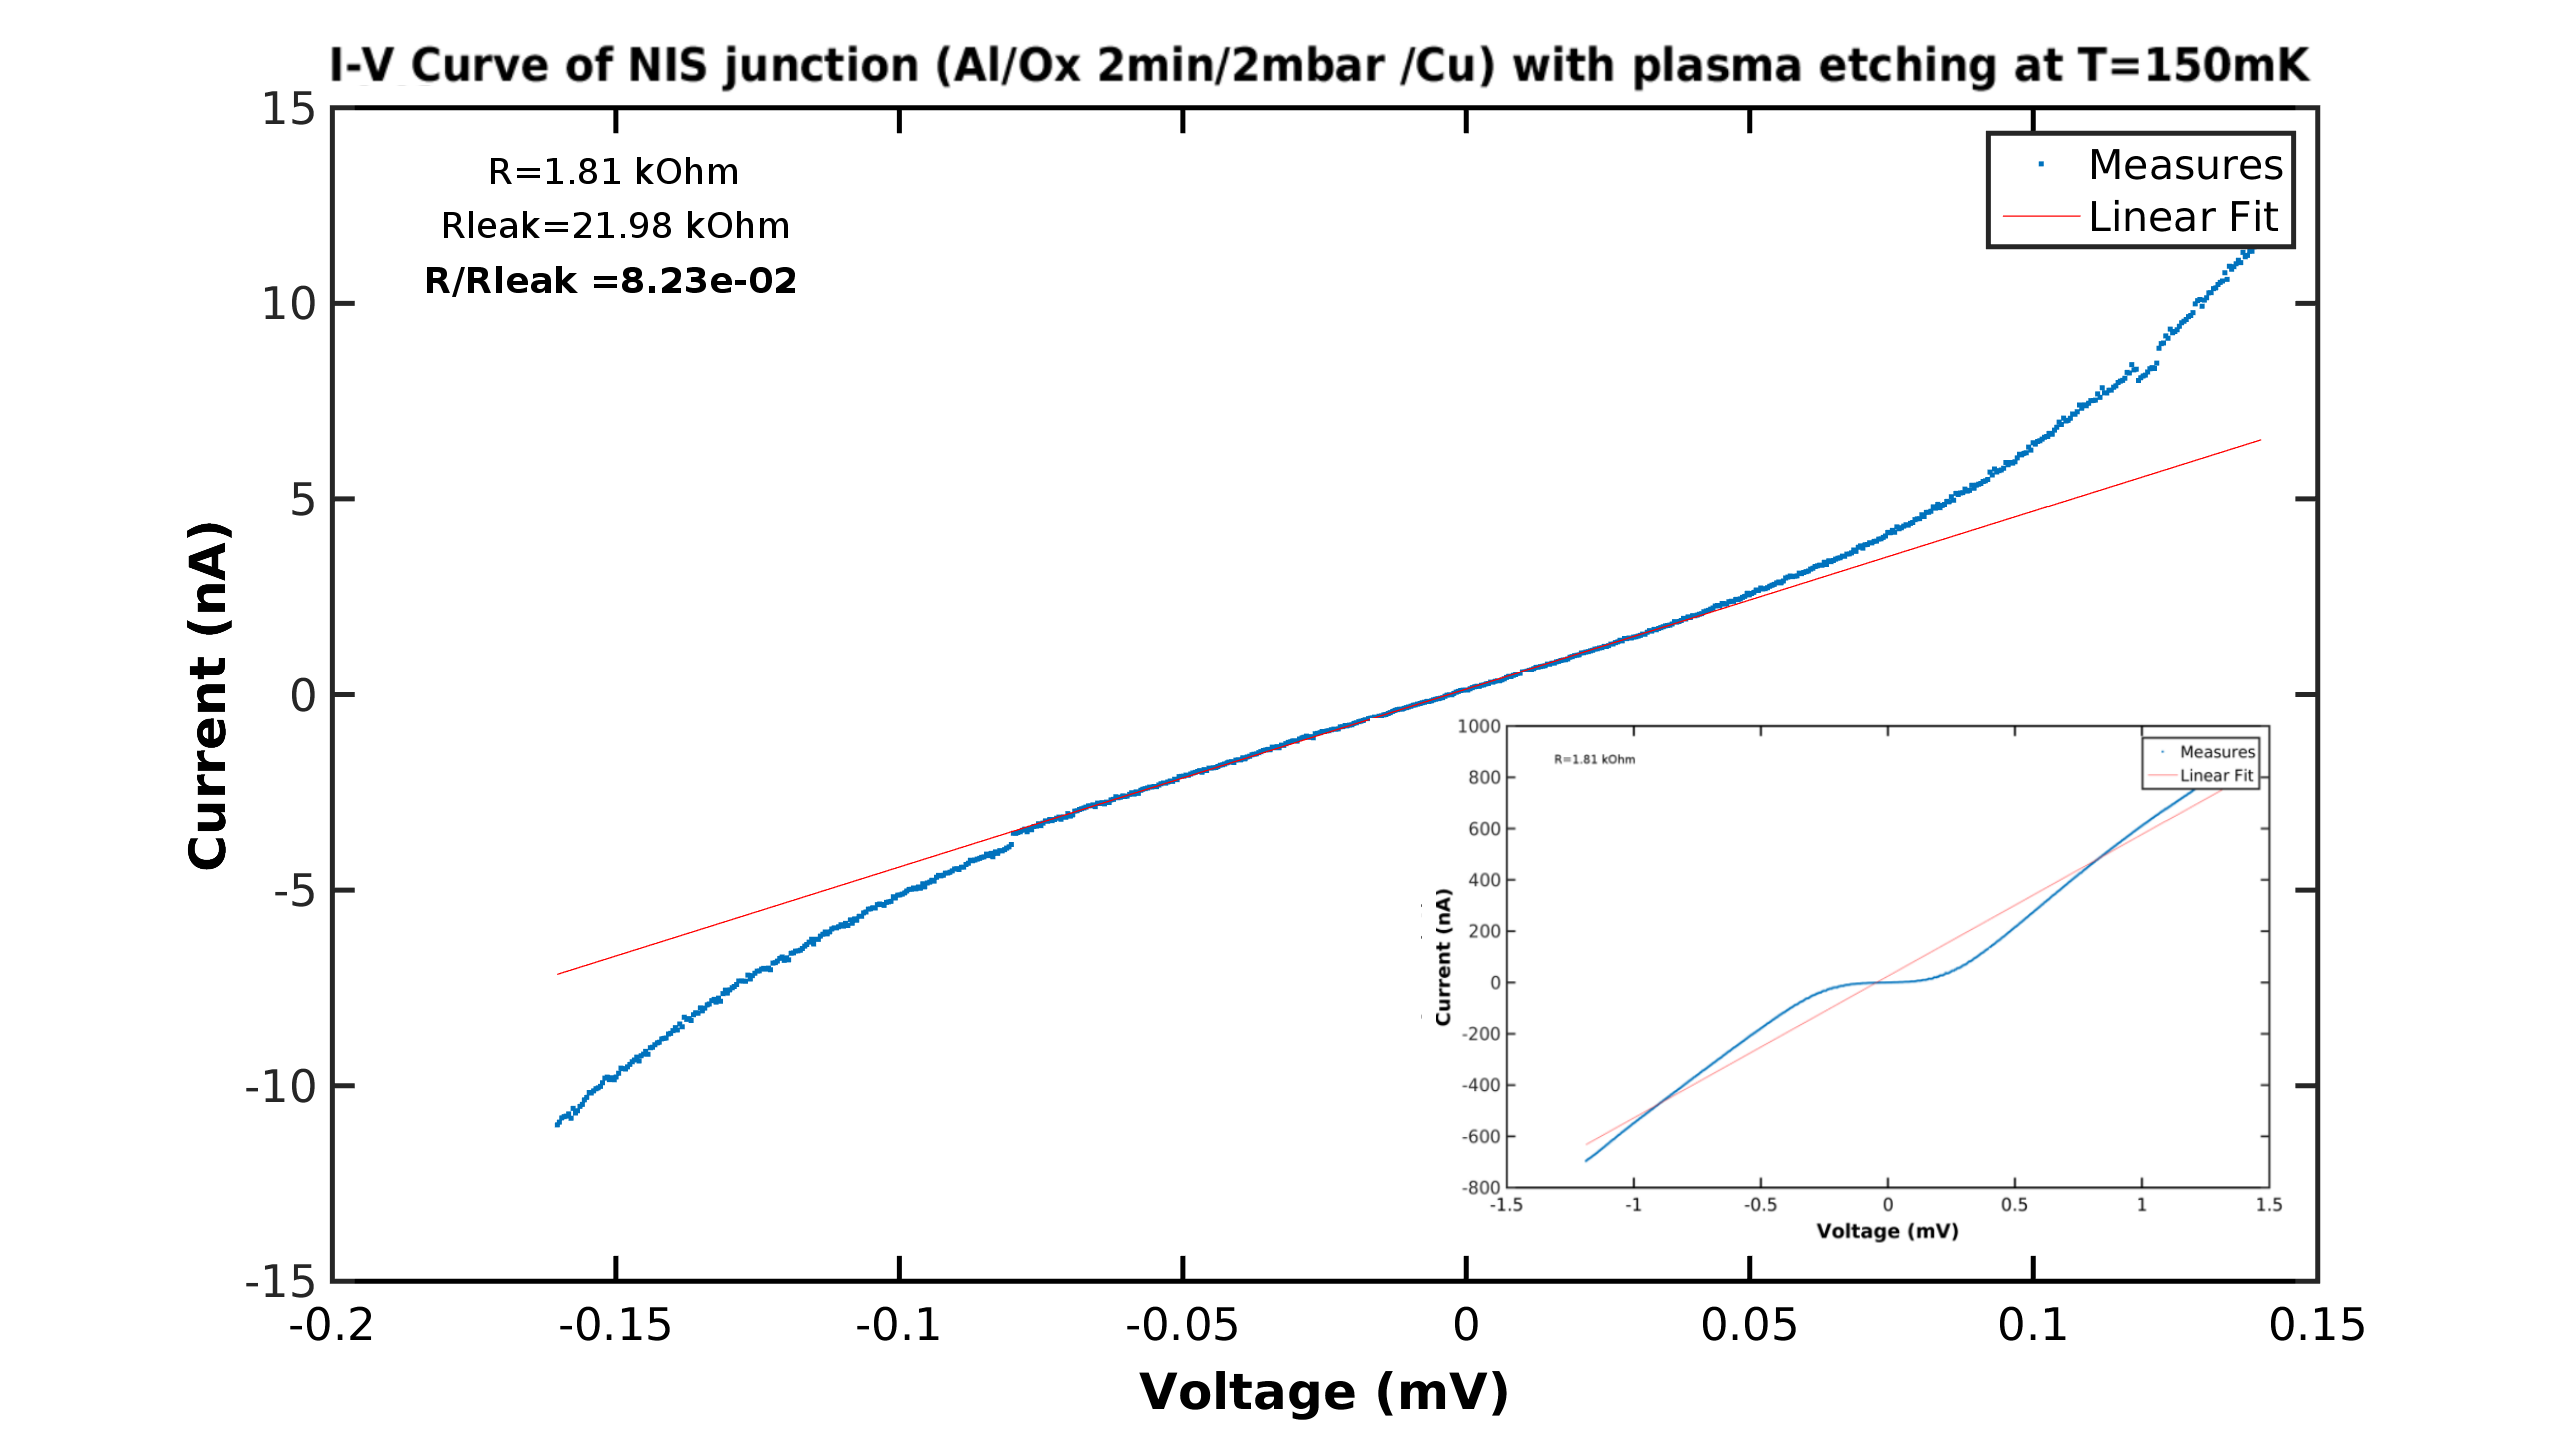
\includegraphics[width=15cm]{PlasmaOx2.png}
            \caption{IV curves of Plasma Etched sample}
            \label{PlasmaOx}
        \end{figure}
           \begin{figure}
            \centering
            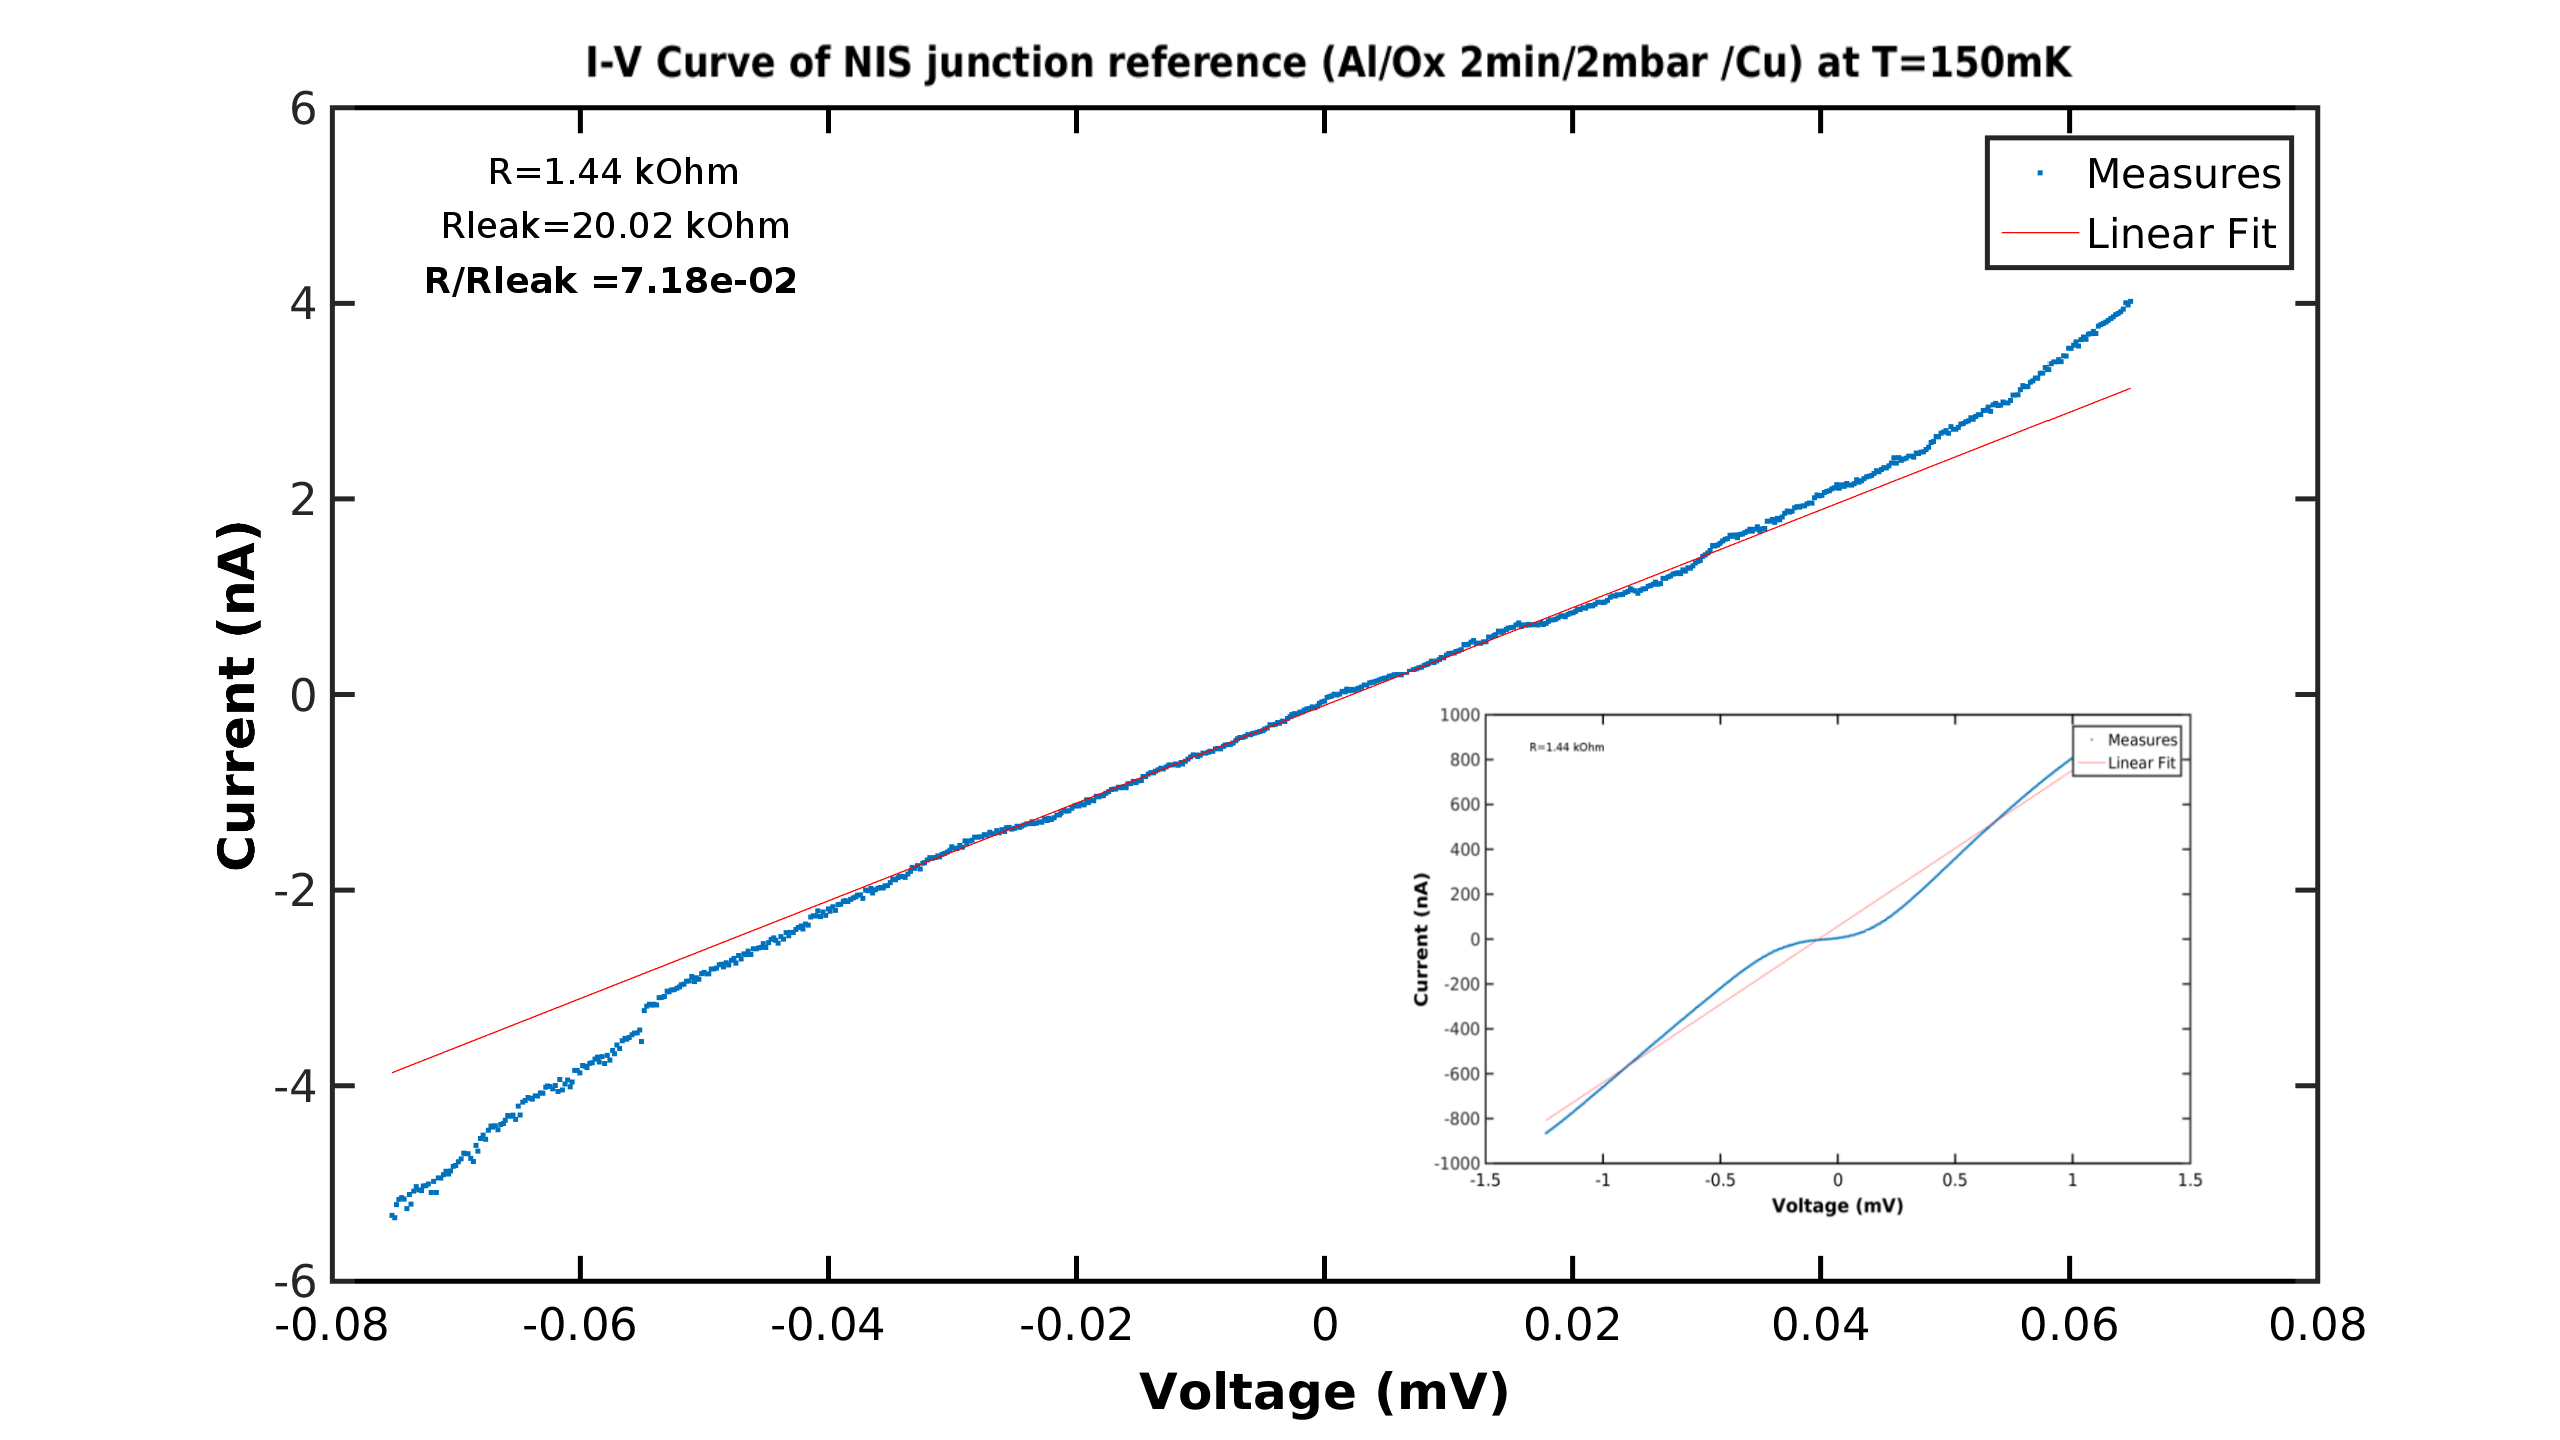
\includegraphics[width=15cm]{RegularOxRef2.png}
            \caption{IV curves of the reference oxidation sample}
            \label{ReferenceOx}
        \end{figure}
           
           We can see that the relation between the current is about the same order of magnitude in both cases : 10$^{-2}$. This is quite a bad result, but since the two relations are about the same value, we could think that the plasma does not damage the junction, but the effect of the plasma etching may be hidden behind the overall poor leakage of all the samples.
                
                \section{Summary of the results}
            
            Plasma etching is working fine, and can etch all the aluminium oxide without any visible damages on the junctions, plus the position of the sample on the sample stage does not affect the behaviour of the plasma etching. The question that has to be solved now is the effect of the plasma on the general quality of the junctions made in the evaporator : after heavy uses of the plasma, the quality of the junctions, in general, have degrading. Is it a coincidence or is it a collateral effect of the plasma ? This has to be solved but still not clear.
                
                

\chapter*{Conclusion}
\addcontentsline{toc}{chapter}{Conclusion}


\bibliographystyle{unsrt}
\bibliography{Bibliography}
\appendix
\chapter{First measurement method}

\section{Bad pattern}
\label{badtests}

We first used a two pad pattern, which is not very practical to make 4 probe measurements, since I either had to put two needles of the probestation on one pad or bound samples stage pad to one another. We finished the samples that were already written with EBL and the we switched to 4 pads patterns.


\section{Bad way of measuring}
\label{badmeasures}
At the beginning, with the 2 pads samples and with the first 4 pads samples, I bounded the samples to a sample stage to measure them with a complicated Matlab assisted setup.
\chapter{Failed Samples}
\section{Failure due to plasma}
\label{badplasma}
The plasma sometimes had some troubles and did not work properly. In the report there were the good samples but the plasma often burned the resist so that the copper evaporation could not be done properly.

\section{Failure due to EBL}
The first EBL writting we made with the 4 pad pattern failed, there was a height problem. The wafer was not complete so it could not be clamped properly with the regular clamps, we had to had another one, which we forgot. The writting was really not usable as we saw with the first evaporation. Of course, we made another one to check that the problem really came from the EBL writting and not from the LISA.
\chapter{Parameters table of the samples}
\label{parametertable}

\begin{tabular}{|c|c|c|c|c|c|}

        \hline
        \textsc{Test n\textdegree}&\textsc{Strong}&\textsc{Plasma}&\textsc{Regular}&\textsc{Comment}\\
        &\textsc{Oxidation}&&\textsc{Oxidation}&\\
        \hline
        Test 10&  &&&Failed EBL\\
        \hline
        Test 11&  &&&Failed EBL\\
        \hline
        Test 12&No&No&No&Clean contact reference\\
        \hline
        Test 13.i&Yes&10 min&No&Several positions\\
        \hline
        Test 14.i&Yes&20 min&No&Several positions\\
        \hline
        Test 15&Yes&No&No&Strong Oxidation reference\\
        \hline
        Test 16&No&No&Yes&Reference Sample Test 17\\
        \hline
        Test 17&Yes&10 min&Yes&Resist burned\\
        \hline
        Test 18&Yes&10 min&Yes&Resist burned\\
        \hline
        Test 19&No&No&Yes&Reference Sample Test 18\\
        \hline
        Test 20&Yes&10 min&Yes&Resist burned\\
        \hline
        Test 21&No&No&Yes&Reference Sample Test 20\\
        \hline
        Test 22&Yes&5 min&No&\\
        \hline
        Test 23&Yes&2 min 30s&No&\\
        \hline
        Test 24&Yes&10 min&Yes&Etched the wafer\\
        \hline
        Test 25&No&No&Yes&Reference Sample Test 24\\
        \hline
        Test 26&Yes&2 min&Yes&\\
        \hline
        Test 27&No&No&Yes&Reference sample Test 26\\
        \hline
        \end{tabular}
\vspace{0.5cm}

\noindent Parameters : 
\begin{itemize}
    \item Strong Oxidation = 10 min under a pressure of 200 mbar of O$_2$
    \item Regular Oxidation = 2 min under a pressure of 2 mbar of O$_2$
    \item Plasma = Pressure of Ar of 4.10$^{-4}$ mbar, Power=40mA, Extraction=-0.8kV\footnote{Lowered to -0.25kV starting from Test 22}, Ion Energy=1.5kV 
\end{itemize}

\chapter{Compléments de résultats}

\section{Images SEM}

\section{Graphes supplémentaires}

\pagestyle{empty}
\newpage
\section*{Abstract}

\begin{Large}
\textbf{Fabrication and measurements of Normal Metal - Insulator - Superconductor junctions to characterize plasma Etching}
\end{Large}

\vspace{0.3cm}

The goal of this internship is to characterize an etching method that can be performed \textit{in situ} to get rid of an unwanted layer of matter : Plasma Etching. Thus, a fabrication process was put in place in cleanroom in order to make the structures (Normal Metal - Insulator - Superconductor junctions) to measure. This process relies on several cleanroom methods, but particularly on the evaporator that allows metal deposition and plasma etching. The measurements done are mostly resistance and current-voltage measurements both at room and low temperature, reached with a dilution cryostat. The reference samples consists in simple NIS junctions, without plasma etching shows results expected by theory : surface dependance of resistance, tunnel and leakage current... Results and conclusions about plasma etching were bothered by some parameters modification (Oxygen cleaning of the plasma gun). Yet, it is interesting to notice that plasma etching is a valide etching method since it can etch Aluminium Oxide, which is isotropic on all the sample stage surface and which is does not imply any damages in the junctions. This internship could determine several key data about plasma etching in the evaporator and help researcher with a new and characterized method to etch.

Key words : Plasma Etching, Evaporator, NIS junctions, Low temperature measurements.

\section*{Résumé}

\begin{Large}
    \textbf{Réalisation et mesure de jonctions Métal - Isolant - Supraconducteur pour la caractérisation de la gravure par plasma}
\end{Large}

\vspace{0.3cm}

Le but de ce stage est de caractériser une méthode de gravure permettant de retirer \textit{in situ} une couche de matière non souhaitée : la gravure par plasma. Ainsi, un processus de fabrication a été mis en place afin de réaliser des structures (jonctions Métal-Isolant-Supraconducteur) à mesurer, incluant, ou non (échantillons référence), la gravure par plasma. Il s'appuie sur différentes techniques de salle blanche, en particulier l'évaporateur permettant de déposer le metal mais aussi de graver avec le plasma. Des mesures de résistances et des tracés de caractéristiques courant-tension ont été réalisées, à la fois à temperature ambiante et à basse température, atteinte par la biais d'un cryostat à dilution. Les échantillons de référence qui consistent en de simples jonctions sans gravure montrent un comportement conforme à celui attendu par la théorie : dépendance en surface de la résistance, courant tunnel et courant de fuite à basse température... Le nettoyage du pistolet à plasma par oxygène a perturbé les résultats concernant la gravure par plasma. Cependant, on notera que le plasma est capable de graver l'Oxyde d'Aluminium, qu'il est isotrope sur l'ensemble du porte-échantillon, et que les jonctions ne sont visiblement pas endommagées par la gravure. Ce stage a donc permis la caractérisation de plusieurs paramètres concernant la gravure par plasma au sein de l'evaporateur et aide à la recherche grâce à cette technique désormais caractérisée.

Mots clés : Gravure par plasma, Evaporateur, Jonctions NIS, Mesures à basse température.

%
% \section*{Abstract}
%
% \begin{Large}
% \textbf{Fabrication and measurements of Normal Metal - Insulator - Superconductor junctions to characterize plasma Etching}
% \end{Large}
%
% This intership involves the fabrication of Normal Metal - Insulator - Superconductor junctions, in cleanroom, and measurements on these samples in order to characterize \textit{in situ} plasma etching of Aluminium Oxide. The goal is to give access to an etching method that can be performed \textit{in situ} to get rid of an unwanted layer of matter (Native Oxide, protecting layer...). Thus, a fabrication process was put in place in cleanroom in order to make the structures to measure. This process relies on several cleanroom methods, but particularly on the evaporator that allows metal deposition and plasma etching. The measurements done are mostly resistance and current-voltage measurements both at room and low temperature, reached with a dilution cryostat. The reference samples consists in simple NIS junctions, without plasma etching shows results expected by theory : surface dependance of resistance, tunnel and leakage current... Results and conclusions about plasma etching were bothered by some parameters modification (Oxygen cleaning of the plasma gun). Yet, it is interesting to notice that plasma etching in a valide etching method since it can etch Aluminium Oxide, that is isotropic on all the sample stage surface and that is does not imply any damages in the junctions. This internship could determine several key data about plasma etching in the evaporator and help researcher with a new and characterized method to etch.
%
%
% \section*{Résumé}
%
% \begin{Large}
%     \textbf{Réalisation et mesure de jonctions Metal - Isolant - Supraconducteur pour la caractérisation de la gravure par plasma}
% \end{Large}
%
% Ce stage met en jeu la fabrication en salle blanche de jonctions Metal - Isolant - Supraconducteur, puis la réalisation de mesures sur ces échantillons en vue de la caractérisation de la gravure par plasma \textit{in situ} d'Oxyde d'Aluminium. Le but est ainsi de permettre le développement d'une méthode de gravure permettant de retirer \textit{in situ} une couche de matière non souhaitée (Oxyde natif, couche protectrice...). Ainsi, un processus de fabrication a été mis en place afin de réaliser les structures à mesurer, incluant, ou non (échantillons référence), la gravure par plasma. Ce processus s'appuie sur les différentes techniques de salle blanche disponibles, en particulier l'évaporateur permettant de déposer le metal mais aussi de graver avec le plasma. Les mesures réalisées sont principalement des mesures de résistances et du tracé de caractéristiques courant-tension, à la fois à temperature ambiante et à basse température, atteinte par la biais d'un cryostat à dilution. Les échantillons de référence consistent en de simples jonctions, sans gravure par plasma et montrent un comportement conforme à celui attendu par la théorie : dépendance en surface de la résistance, courant tunnel et courant de fuite à basse température... Les résultats concernant la gravure par plasma ont été perturbés par changement de paramètres (nettoyage par oxygène du pistolet à plasma) au cours du stage. Cependant, il est intéressant de noter que le plasma est capable de graver l'Oxyde d'Aluminium, qu'il est isotrope sur l'ensemble du porte-échantillon, et que les jonctions, ne sont visiblement pas endommagées par la gravure. Ce stage a donc permis la caractérisation de plusieurs paramètres concernant la gravure par plasma au sein de l'evaporateur et aide à la recherche grâce à une technique désormais caractérisée, pour graver.
%

\end{document}
